%% Dokumentklasse %%

  \documentclass[a4paper, halfparskip-, bibtotoc, pointednumbers, openbib]{scrartcl}

%% Pakete %%

  \usepackage[a4paper,left=2.5cm,right=2.5cm,top=2cm,bottom=4cm]{geometry}         	%% Seitenr�nder
  \usepackage[latin1]{inputenc}                                                     %% ISO-Text mit Umlauten
  \usepackage[T1]{fontenc}                                                          %% Zeichensatz mit Umlauten
  \usepackage[german]{babel}                                                       %% BABEL -> german , neue Rechtschreibung
  \usepackage[dvips]{graphicx}
  \usepackage[dvips]{rotating}
  \usepackage{color}
  \usepackage[reqno, fleqn]{amsmath}
  \usepackage{longtable}
  \usepackage{varioref}
  \usepackage{multicol}
	\usepackage{units}
 % \usepackage{verbatim}
  \usepackage{lscape}
  \usepackage{float}
 % \usepackage[light,outline]{draftcopy}
 % \usepackage{natbib}

%%%%%%%%% HARVARD STYLE CITATION -> remove each one % (comment marker) per line %%%%%%%%%%%%
%% round parantheses for Literature, taken from https://tex.stackexchange.com/questions/240741/references-numbering-in-parenthesis-using-thebibliography
%% Change appearance of numeric labels in citation call-outs
%\usepackage{cite}
%\renewcommand\citeleft{(}
%\renewcommand\citeright{)}
%% Change appearance of numeric labels in bibliography 
%\makeatletter
%%\renewcommand{\@biblabel}[1]{(#1)}
%\renewcommand{\@biblabel}[1]{~}   % <-- set nothing as prefix (just list items)
%\makeatother

  \usepackage{array}
  \usepackage{tabularx}
	  \newcolumntype{Y}{>{\center\arraybackslash}X}
  \usepackage{multicol, multirow, calc, array} % Tabellen manipulieren
  %\usepackage{ragged2e}
  \usepackage{calc}
  \usepackage{amsmath, amssymb, amsfonts} % Mathebibliotheken

  \usepackage[table]{xcolor}
	

  \usepackage{bm}
 % \usepackage{palatino}
  \usepackage{lmodern}
 % \usepackage{mathptmx}
 % \usepackage{helvet}
 % \usepackage{courier}

  \usepackage[automark]{scrpage2}
  \usepackage[margin=30pt,tableposition=top,labelfont={sf,bf},font=small]{caption}             %% Tabellen und Abbildungs�berschriften
	  %\usepackage{subfig}
	%\usepackage[list=true, font=large, labelfont=bf, labelformat=brace, position=top]{subcaption}
	\usepackage[margin=0pt,size=smaller,labelformat=parens,labelsep=space,skip=6pt,list=true,hypcap=false]{subcaption}
	\captionsetup[subfigure]{margin=0pt,size=smaller,labelformat=parens,labelsep=space,skip=6pt,list=true,hypcap=false}
	\usepackage[pdfpagelabels,linktocpage,colorlinks,linkcolor=blue,citecolor=magenta,bookmarksnumbered]{hyperref} %% Hyperlinks im PDF
  \usepackage{hypcap}                                                                          %% Korrekte Bild-Referenz

  \usepackage{graphicx}
	\usepackage{comment}
	\usepackage{soul}
  \usepackage{epstopdf}
	
	%\usepackage{ulem}
	\usepackage{color}
	\usepackage{listings}

	\usepackage{ifthen}

%% Definitionen %%

   %%%%%%%%%%%%%%%%%%%%%%%%%%%%%%%%%%%%%%%%%%%%%%%%%%%%%%%%%%%%%
   %%  Abstand Oberer Bildrand-Abbildung
   %%
      \renewcommand\hypcapspace{\baselineskip}
   %%%%%%%%%%%%%%%%%%%%%%%%%%%%%%%%%%%%%%%%%%%%%%%%%%%%%%%%%%%%%


%   %%%%%%%%%%%%%%%%%%%%%%%%%%%%%%%%%%%%%%%%%%%%%%%%%%%%%%%%%%%%%
%   %%  PDF Optionen
%   %%
%      \hypersetup{
%        pdftitle={TSM1 - 1.Hausaufgabe},
%        pdfauthor={Georg Walde},
%        pdfsubject={Hausaufgabe 1},
%        pdfproducer={ps2pdf},
%        pdfcreator={Latex}
%      }
%   %%%%%%%%%%%%%%%%%%%%%%%%%%%%%%%%%%%%%%%%%%%%%%%%%%%%%%%%%%%%%


%   %%%%%%%%%%%%%%%%%%%%%%%%%%%%%%%%%%%%%%%%%%%%%%%%%%%%%%%%%%%%%
%   %%  Move numbers of section headings left into the margin
%   %%
%   %% Re-define \chapterformat only if it is defined and not
%   %% \relax without making it \relax if it is not defined:
%      \begingroup
%      \expandafter\expandafter\expandafter\endgroup
%      \expandafter\ifx\csname chapterformat\endcsname\relax\else
%        \renewcommand*{\chapterformat}{%
%          \llap{%
%            % Following line is the original definition
%            \chapappifchapterprefix{\ }\thechapter\autodot\enskip
%          }%
%        }
%      \fi
%
%      % Re-define \othersectionlevelsformat
%      \renewcommand*{\othersectionlevelsformat}[1]{%
%        \llap{%
%          % Following line is the original definition
%          \csname the#1\endcsname\autodot\enskip
%        }%
%      }
%   %%
%   %%  End of redefining format makros
%   %%%%%%%%%%%%%%%%%%%%%%%%%%%%%%%%%%%%%%%%%%%%%%%%%%%%%%%%%%%%%




\pagestyle{scrheadings}
      \clearscrheadfoot
%       \ihead{\headmark}
%       \ohead{\pagemark}
        \ofoot{\ifnum \value{page}>1 \thepage \fi}
				\definecolor{lightgray}{gray}{0.6}
				\definecolor{cell-lightgray}{gray}{0.95}
				\ifoot{\color{lightgray} \scriptsize \upshape
				Dominik Woelki, Berlin Moabit\\
				 \textit{https://github.com/dwoelki}
				}

%   %%%%%%%%%%%%%%%%%%%%%%%%%%%%%%%%%%%%%%%%%%%%%%%%%%%%%%%%%%%%%
%   %% Neubeginn der Gleichungsnummerierung am Kapitelanfang
%   %%
%      \numberwithin{equation}{chapter}
%   %%%%%%%%%%%%%%%%%%%%%%%%%%%%%%%%%%%%%%%%%%%%%%%%%%%%%%%%%%%%%


   %%%%%%%%%%%%%%%%%%%%%%%%%%%%%%%%%%%%%%%%%%%%%%%%%%%%%%%%%%%%%
   %% �nderung der Tabellenparameter
   %%
      \setlength{\arrayrulewidth}{0.5pt}
      \renewcommand{\arraystretch}{1.3}
   %%%%%%%%%%%%%%%%%%%%%%%%%%%%%%%%%%%%%%%%%%%%%%%%%%%%%%%%%%%%%


   %%%%%%%%%%%%%%%%%%%%%%%%%%%%%%%%%%%%%%%%%%%%%%%%%%%%%%%%%%%%%
   %% Aussehen der enumerate-Zahlen
   %%
      \renewcommand\labelenumi {\sffamily{\bfseries{\theenumi.}}}
   %%%%%%%%%%%%%%%%%%%%%%%%%%%%%%%%%%%%%%%%%%%%%%%%%%%%%%%%%%%%%


   %%%%%%%%%%%%%%%%%%%%%%%%%%%%%%%%%%%%%%%%%%%%%%%%%%%%%%%%%%%%%
   %% Nummerierung und Unterschriften von subfigures
   %%
%%%%%%%%%%%%%%%%%%%%%%%%%%%%%%%%%%%   KOMMENTIERT DW 2020-03-04, WEIL ANDERES PACKAGE BENUTZT      \captionsetup[subfloat]{listofformat=subsimple, labelformat=simple, labelsep=colon}
     % \renewcommand\thesubfigure {\thefigure \thinspace \alph{subfigure}}
      \renewcommand\thesubfigure {\alph{subfigure}}
   %%%%%%%%%%%%%%%%%%%%%%%%%%%%%%%%%%%%%%%%%%%%%%%%%%%%%%%%%%%%%


%   %%%%%%%%%%%%%%%%%%%%%%%%%%%%%%%%%%%%%%%%%%%%%%%%%%%%%%%%%%%%%
%   %% Tiefe der Verzeichnisses anpassen
%   %%
%     \setcounter{secnumdepth}{4}
%     \setcounter{tocdepth}{4}
%     \setcounter{lofdepth}{2}
%   %%%%%%%%%%%%%%%%%%%%%%%%%%%%%%%%%%%%%%%%%%%%%%%%%%%%%%%%%%%%%


%   %%%%%%%%%%%%%%%%%%%%%%%%%%%%%%%%%%%%%%%%%%%%%%%%%%%%%%%%%%%%%
%   %%  Draftcoppy ab Seite 2
%   %%
%      \draftcopyFirstPage{2}
%   %%%%%%%%%%%%%%%%%%%%%%%%%%%%%%%%%%%%%%%%%%%%%%%%%%%%%%%%%%%%%



%\includeonly{Vorlage_muster}

%%%\begin{document}

\pagenumbering{Roman}		%Beginn mit r�mischen Seitenzahlen




										
\begin{document}
			%----------------------------------------------
			%
			%									INSTITUTSSYMBOL
			%
			%----------------------------------------------	

\hspace*{-2.5cm}															  % gesamte Titelseite um 1cm nach rechts verschieben
\parbox[t][21cm][t]{3.5cm}										% zwischen den parbox'n darf keine Leerzeile existieren
	{																						% sonst werden sie untereinander statt nebeneinander gestellt	
		\begin{center}
			\vspace*{-1cm}
			\hspace*{1cm}
			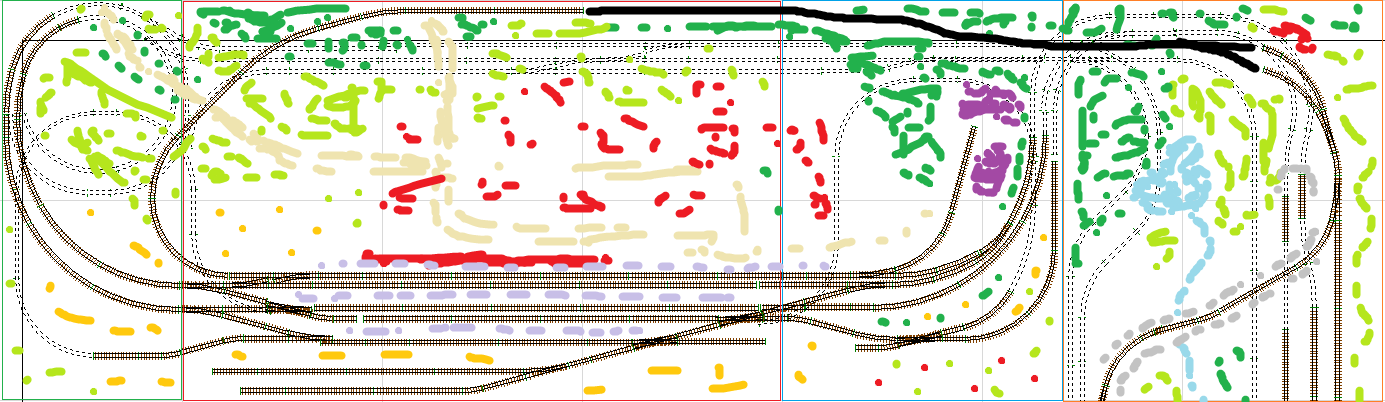
\includegraphics[scale=0.5]{img/cover}		% LOGO des LA
		\end{center}
	}
\begin{sf}
			%----------------------------------------------
			%
			%						INSTITUTSNAME UND PROFESSOR
			%
			%----------------------------------------------	
\parbox[t][22cm][t]{12cm}											% parbox = 2.Spalte mit Text
			  {																			% [Ausrichtung] [H�he] [AusrichtenInnen] {Breite}
			  	\begin{flushleft}
					  \vspace*{-0.3cm}									% (2-x)cm = Abstand zwischen ITS-Logo und -Name
				    \hspace*{8cm}
				    \parbox[t][3.0cm][t]{12cm}				
									{
										%Dominik Woelki\\
										%Berlin\\
									}
						
			%----------------------------------------------
			%
			%									TITLE
			%
			%----------------------------------------------		
						\vspace{4cm}														% Leerzeile vor vertikaler Abstandsangabe notwendig
						\parbox[t][0.5cm][t]{12cm}									% [Ausrichtung] [H�he] [AusrichtenInnen] {Breite}
							{
								\centering
								 {
								   \textbf{\Huge{
												\centerline{Granitz}
												}}\\
								 }  
							}\\
			%----------------------------------------------
			%
			%									SUB TITLE
			%
			%----------------------------------------------		
						\vspace{4.5cm}														% Leerzeile vor vertikaler Abstandsangabe notwendig
						\parbox[t][2cm][t]{12cm}									% [Ausrichtung] [H�he] [AusrichtenInnen] {Breite}
							{
								\centering
								 {
									%\large{
								   \textbf{\LARGE{
										\centerline{Modelleisenbahnanlage}
										\centerline{Spur N}
										}}
%S									\includegraphics[scale=1.0]{img/IPSM_splash_new.jpg}
										%}
								 }  
							}				
				
				
		 %----------------------------------------------
		 %
		 %									BOOK
		 %
		 %----------------------------------------------				
						 \vspace{1.0cm}															% Leerzeile vor vertikaler Abstandsangabe notwendig
						 \parbox[t][3cm][t]{12cm}
								{
									\centering
												\textbf{\LARGE{
												\centerline{Story \& Dokumentation}%\\
												%\centerline{Disk Temperature Model}
												}
												}\\
					  		} 		
					  \end{flushleft}


		
		 %----------------------------------------------
		 %
		 %							BETREUER und DATUM
		 %
		 %---------------------------------------------- 		  
						\vspace*{2.0cm}
						\parbox[t][1cm][t]{4cm}				
							{
								\leftline{\Large Dominik Woelki}
								\vspace*{0.5cm}
								%\hrule
								\vspace*{0.5cm}
								%\leftline{\Large \today}
								\begin{tabular}{p{.25\textwidth-2\tabcolsep} p{.6\textwidth-2\tabcolsep}}
								\hline
								 & \\
								%\Large \today & version: related to IPSM dev1.4
								\Large \today & 
								\end{tabular}
							}
 }	% end parbox (2.Spalte mit Text)
\end{sf}

\clearpage


\newboolean{INTERNAL_VERSION}
\setboolean{INTERNAL_VERSION}{false}

\ifthenelse{\boolean{INTERNAL_VERSION}}{

	\section*{NOTE TO REVIEWERS}
	
	\begin{table}[h]
	\begin{tabular}{||l||}
	\hline
	\textbf{Highlighted text (\hl{this way}) is either meant to be for internal version only}\\
	\textbf{and to be removed for version to be published \textit{or} information to be verified.}
	\\	
	If a parameter name of a table's column is highlighted, the entire column will be removed.\\
	Same applied to a table's line, if the line's first cell is highlighted.
	\\
	If the entire caption of a figure is highlighted, the entire figure will be removed.\\
	If single sub-figure captions (within a minimap) are highlighted, only these sub-figures will be removed.
	\\
	\hline
	\end{tabular}
	\end{table}
	
}{
	
	\section*{Vorbemerkungen zur Verwendung des Dokuments}
	
	Diese Dokumentation ist ein Freizeitwerk und handelt ein Hobby ab, in dem der Spa{\ss} im Mittelpunkt stehen soll.
	Der Autor ist ein Dokumentationsfetischist, um Entwicklungen festzuhalten (d.h. Versionierung, auch im strengen Sinne!) und Wissen zu teilen.
	Dem Autor geht es dabei allgemeinhin nicht um Selbstdarstellung, sondern Wissenstransfer und Aufmunterung zur Zusammenarbeit.
	KollegInnen k\"onnen das i.d.R. best\"atigen.
	
	Der Autor spricht aus Gewohnheit h\"aufig von sich in der dritten Person.
	Er h\"alt sich aber nicht f\"ur Julius Caesar.
	Die personalisierte Schreibform geh\"ort einfach nicht in den beruflichen Alltag, wenn es um Dokumentation geht.
	Hier und da erinnert sich der Autor daran, so dass gelegentlich das 'Ich' in Erscheinung tritt.
	
	Text, der \hl{in dieser Art gehighlighted} ist, markiert entweder unverifizierten Inhalt, der zu einem sp\"ateren Zeitpunkt einem entsprechenden Review unterzogen wird, oder (noch) unvollst\"andigen Inhalt.
	Die Dokumentationssprache ist Deutsch.
	Sporadisches Aufflammen eines gewissen Denglisch ist wiederum dem Berufsalltag geschuldet.
	Separierte Dokumentationen von mir, die sich mit sp\"ater eingesetzter, selbst geschriebener Software oder Hardwareansteuerung befassen, sind i.d.R. in Englisch dokumentiert.
	Sorry, als Dokumentationssprache ist Englisch heutzutage einfach sinnvoller.
	Was die Modellbahn selbst betrifft, bleibe ich lieber zu Hause oder zumindest in der Region.
	Von daher ist das noch ein sinnvoller Bereicht f\"ur deutschsprachige Dokumentation.
	Au{\ss}erdem haben Amerikaner tendenziell andere Vorstellungen davon, wie ein Zug aussehen sollte, als ich.
	
	Die Angaben in dieser Dokumentation spiegeln mal mehr, mal weniger abstrakt Ansichten des Autors wider.
	Auch f\"ur den Fall, dass einige Passagen, insbesondere was Lokalpatriotismus und das regionale Umfeld des modellierten Szenarios betrifft, etwas bissig erscheinen, so sind sie niemals b\"oser Natur.
	Der Autor ist zuallererst begr\"u{\ss}ender Weltb\"urger, danach erst Berliner und Europ\"aer.
	Die Staatlichkeit spielt f\"ur ihn sehr untergeordnete Rolle.
	Der Autor begr\"u{\ss}t alle nicht menschenverachtenden Lebensmodelle.
	
	Die Dokumentation wird unentgeltlich zur Verf\"ugung gestellt und ich erhalte von niemandem daf\"ur eine Verg\"utung in welcher Form auch immer.
	Die Nennung von Marken, die im Modelleisenbahnbau g\"angig sind, sind nicht als Werbung an sich zu verstehen, sondern sollen Aufschluss \"uber verwendete Baus\"atze und Zugmaterial geben.
	Die genannten Marken sind i.d.R. eingetragene, gesch\"utzte Markennamen.
	Alle Bemerkungen zu deren Sortimenten sind rein zweckgebunden und in keinem Fall allgemein-wertend zu verstehen.
	Alle genannten Modelleisenbahnhersteller (und dar\"uber hinaus noch viel mehr) sind meiner Meinung nach per se einem gewissen Idealismus verschrieben, so dass ihre Daseinsberechtigung und ihre Sortimente unsere Hobbywelt bereichern.
	
	Die Dokumentation wird zur Verf\"ugung gestellt, wie sie als jeweiliges PDF-Dokument kompiliert ist (\textit{'as is'}).
	Die Selbstkompilierung oder anderweitige Nutzung von Rohdateien erfolgt auf eigene Verantwortung.
	Dies betrifft den vollst\"andigen Umfang des Git-Projekts, das unter folgendem Link abrufbar ist:
	\begin{itemize}
		\item[] \textit{https://github.com/dwoelki/Granitz\_Documentation}
	\end{itemize}
	Der Autor \"ubernimmt keine Haftung f\"ur Sch\"aden, die durch die Dokumentation \textit{as is} oder Folgesch\"aden, z.B. durch Nachbau, entstehen.
	Der Autor \"ubernimmt generell keine Haftung und Garantie f\"ur irgendwelche Teile dieser Dokumentation.
	Verlinkte Inhalte werden nach bestem Wissen und Gewissen auf Legalit\"at und politische Korrektheit \"uberpr\"uft.
	Gleichwohl \"ubernimmt der Autor keine Haftung f\"ur verlinkte Inhalte.
	
	Das Dokument sowie das gesamte Git-Repository mit Quell- und Erg\"anzungsdateien sind unter der \textit{Apache 2.0 License} lizensiert \cite{Apa04}.
	Der vollst\"andige Text der Lizenz als Template, zu erg\"anzen um den Namen des Autors, ist verf\"ugbar unter folgendem Link:
	\begin{itemize}
		\item[] \textit{https://www.apache.org/licenses/LICENSE-2.0.txt}
	\end{itemize}
	
	Dar\"uber hinaus gelten alle Konditionen der Apache 2.0 License.
	
}

\clearpage



\tableofcontents
\newpage
\listoffigures
\listoftables

\newpage

\section*{Nomenclature}
\textbf{Symbols:}\\
	\begin{tabular}{p{.15\textwidth-2\tabcolsep} p{.15\textwidth-2\tabcolsep} p{.7\textwidth-2\tabcolsep}}
		$\Delta$ & & Difference \\
		$\underline{x}$ & & Guess Vector \\
	\end{tabular}
\\

%\newpage
\noindent
\textbf{Indices:}\\
	\begin{tabular}{p{.25\textwidth-2\tabcolsep} p{.75\textwidth-2\tabcolsep}}
		' & Null Dimensional \\
	\end{tabular}
\\

%\newpage

\noindent 
\textbf{Abbreviations:}\\
	\begin{tabular}{p{.25\textwidth-2\tabcolsep} p{.75\textwidth-2\tabcolsep}}
		$\Psi$-Core & IPSM PSI-Core \\
	  BR & Baureihe \\
		DB & Deutsche Bundesbahn \\
		DBAG & Deutsche Bahn AG \\
		DR & Deutsche Reichsbahn \\
		DWRRC & DWRasp-Rail-Controller \\
		EC & Eurocity \\
		GPIO & General Purpose Input Output \\
		IC & Intercity \\
		ICE & Intercity-Express \\
		IDE & Integrated Development Environment \\
		ILR & Institut f\"ur Luft- und Raumfahrt der Technischen Universit\"at Berlin \\
		IPSM & Interface for Performance and Secondary Air System Modeling \\
		IR & Interregio \\
		IRC & Internet Relay Chat \\
		JWD & Janz Weit Drau{\ss}en \\
		LAN & Local Area Network (z.B. Heimnetzwerk) \\
		RB & Regionalbahn \\
		RE & Regionalexpress \\
		WLAN & Wireless Local Area Network \\
		\\
		\\
		\\
		Abb. & Abbildung \\
		Kap. & Kapitel \\
		Tab. & Tabelle \\
	\end{tabular}
	
\noindent 

	
\clearpage
\pagenumbering{arabic}		% Umbruch zu arabischen Seitenzahlen



\setcounter{section}{-1}

	\section*{Abstract}
\label{sec:abstract}

Dieses Dokument beschreibt die Hintergrund- und Entstehungsgeschichte der privaten Modelleisenbahnanlage Granitz.
Das Thema der Anlage ist die fiktive Stadt Granitz, die in Brandenburg, tendenziell s\"udwestlich von Berlin lokalisiert ist.
Granitz liegt an einer zweigleisigen Hauptsrecke, die einen gut frequentierten Regionalverkehr sowie einige Fernverkehrsverbindungen anbietet.
Die Stadt ist im RE und RB Betrieb routinem\"a\"siger Haltepunkt zwischen Berlin und dem etwa gleich gro\"sen fiktiven Ort Schattenwalde.

Das Szenario ist zeitlich in Epoche V verordnet.
Hier nimmt es aber auch die komplette Bandbreite ein:
War Granitz um die Wende herum noch eine belebte Stadt mit angesiedelter Industrie und regem G\"uterverkehraufkommen im St\"uckverkehr, so ist es in den 2000ern vergessen worden.
Erkl\"artes Ziel der Anlage ist es daher auch, beide Zust\"ande abzubilden, sowohl betrieblich als auch im Diorama.
Letzteres soll relativ einfach durch Austausch weniger, gestalterischer Anlagenelemente erfolgen.

Die komplette Anlage ist auf Normalspur in Spur N, Ma\"sstab \textit{1:160} ausgef\"uhrt.
Bei dem Gleissystem handelt es sich um das Stecksystem Arnold N.
Der Betrieb ist analog.
Eine computergest\"utzte Blocksteuerung und somit weitestgehende \"uber PC and ggf. Smartphone einstellbare Teilautomatisierung ist vorgesehen.

  \section{Einleitung}
\label{sec:introduction}

\subsection{\"Uber den Autor}
\label{sec:author}

Der Autor entstammt einer alteingesessenen, Westberliner Familie und ist irgendwann in den 80ern geboren.
So wichtig dieser Lokalpatriotismus dem Autor auch ist, so stark bef\"urwortet er und bewegt ihn auch das Zusammenwachsen mit dem \"ubrigen Ostdeutschland.
Ostberliner und Brandenburger waren seit der fr\"uhen Jugend immer in gro{\ss}er Zahl im Freundeskreis vertreten.

Die Mauer ist tats\"achlich nur eine sehr d\"unne Erinnerung.
Dennoch waren die Grenzkontrollen im Familienurlaub immer sehr beeindruckend und wurden auch auf den mit dem Bruder gezeichneten Spielstra{\ss}en z.T. verarbeitet.
In Sachsen gab es auch einen Ableger der Familie.
Onkel Kurt's Modelleisenbahnanlage war legend\"ar, war sie szenisch doch unglaublich ausgebaut und zudem praktisch, an die Wand klappbar untergebracht.
In der engen Familie selbst hatten wir auch mehrere Anlagen (Vater, Mutter, Bruder und der Autor; nur die Schwester konnte sich nie daf\"ur interessieren).
Diese gingen nur sp\"arlich \"uber das Stadium der Gleisw\"uste hinaus.
Pl\"ane zur Ausgestaltung gab es immer viele, realisiert wurden aber nur einige H\"auseraufstellungen sowie aufgeklebte Stra{\ss}en.
Spielspa{\ss} haben sie trotzdem viel geboten.

Sp\"atestens im 14. Lebensjahr muss das Interesse an der Modellbahn verloren gegangen sein.
Dazu kam einige Jahre sp\"ater ein gr\"o{\ss}erer Umzug.
Die eigene Platte ist in den Keller des Vaters abgewandert und dort zwei Jahrzehnte verblieben - tats\"achlich aber ohne zu verrotten.
Pers\"onlich ist in der Zeit viel passiert.
Inzwischen ist man beruflich im Ingenieurbereich unterwegs und Simulation geh\"ort zum daily business.
Der Autor ist ausdr\"ucklich kein geborener Rumschrauber!

Zu den eigentlichen Hobbies geh\"oren u.a. Laufen und Wandern, was einen auch viel und gern ins Brandenburger Umland bringt, das dann aber doch so v\"ollig anders als das diverse Berlin ist.
Das bringt einen au{\ss}erdem h\"aufig an die so genannten Lost Places, mal mehr, mal weniger bekannt:
verlassene Milit\"areinrichtungen und stillgelegte Bahnstrecken.
Immer im Verfall befindlich.
Dazu die Eisenbahn als sinnvolles und bevorzugtes (neben Fahrrad) Verkehrsmittel ansehen.
Es erscheint dann irgendwie sinnvoll, dass auch die Modelleisenbahn niemals komplett aus dem Blickfeld entschwunden ist.

\subsection{Wiedereinstieg \"uber die V\"aterliche Anlage}
\label{sec:theReturn}

Richtig los ging es wieder um Weihnachten \hl{2015} rum, als der Vater seine Platte f\"ur seine Enkel ausmottete.
Nach all den Jahren hat aber vieles nicht mehr verl\"asslich funktioniert und der Wille zum unter die Platte kriechen war auch nicht da, also hat der Autor und sein Bruder immer wieder mal Hand angelegt.
Das Szenario dieser Anlage muss in den Voralpen und schwerpunktm\"a{\ss}ig in Epoche IV angesiedelt werden, im Fuhrpark etwas auf Epoche II und III erweitert.
Abb.~\hl{XX} zeigt ein Bild der Anlage.

\hl{FIGURE XX}

Seitdem wurde die Idee einer neuen, eigenen Anlage aufgegriffen, ohne zu wissen, wann und wie diese realisiert werden k\"onnte.
Zus\"atzlicher Spirit wurde bei einem besuchten Fahrtag des Pro Sport Berlin 24 e.V. in Berlin Wedding (zwischenzeitlich leider aufgel\"ost) getankt.
Um Weihnachten 2018 rum gab es dann eine ordentliche Instandsetzung der v\"aterlichen Anlage inklusive einiger untergeordneter Gleisplanoptimierungen.
Der Vorsatz war seitdem dreigeteilt:
\begin{enumerate}
	\item Vorbereitung einer Computersteuerung f\"ur die analoge Anlage, inkl. Erarbeitung der hierf\"ur erforderlichen elektrotechnischen Grundlagen
	\item Versuchsweise Ausgestaltung des Diorama's, auch um wesentliche Kenntnisse f\"ur eine sp\"atere Umsetzung des Eigenentwurfs zu erwerben
	\item Review des eigenen Entwurfs
\end{enumerate}
Der Eigenentwurf brachte sogar eine Aufstellung der Anlage beim Vater selbst ins Spiel (allerdings nie in R\"ucksprache...), wodurch ein Anschluss zur v\"aterlichen Anlage angedacht wurde.
Der Name der Stadt, die im Zentrum des Eigenentwurfs steht, war bereits \hl{2015} auf Granitz fixiert worden, eine fiktive Stadt in Brandenburg, wahrscheinlich s\"ud\"oestlich von Berlin Richtung Cottbus gelegen.

Wieder ein Jahr sp\"ater wurde der Eigenentwurf nochmals \"uberarbeitet und viel mit dem Bruder diskutiert.
Durch ein sich ergebendes Zeitfenster ohne berufliche und pers\"onliche Dauerauslastung wurde dann im Januar 2020 der Entschluss gefasst:
Granitz soll umgesetzt werden, egal ob mit oder ohne Platz in der Wohnung.
Durch die eigene Arbeit in der Programmierung stark von Modularisierung gepr\"agt, wurden auch verschiedene Ideen f\"ur eine Segmentierung des Eigenentwurfs durchgesponnen, um die Anlage schnell verstauen zu k\"onnen und verl\"asslich wieder zusammensetzen zu k\"onnen.

Ein weiterer - nat\"urlich v\"ollig unsinniger xD - Schritt zur Forcierung des Unterfangens war der Ankauf von Zugmaterial f\"ur das geplante Szenario.
Ganz nach dem unkonventionellen Motto: Investieren, um Argumente gegen einen schnellen Wiederausstieg zu schaffen.
Oder noch einfacher: Fakten schaffen.
Letzteres wurde mit der gegebenen Vorsicht auch bei der Ehefrau bzgl. des ben\"otigten Platzbedarfs gemacht.
Der Widerstand fiel hier aber quasi aus ...einer von vielen Gr\"unden, weshalb ich mich gl\"ucklich sch\"atzen kann, sie gefunden zu haben.



\subsection{Epoche V und Brandenburg als Thema}
\label{sec:theme}

Die Erinnerungen an die ersten Jahre nach der Wende und damit auch immer h\"aufiger werdenden Ausfl\"uge ins ehemalige Ostberlin oder umgebende Brandenburg haben bis heute einen tiefen Eindruck hinterlassen:
Von Anfang an war das f\"ur ein Kind gew\"ohnungsbed\"urftig und erschien auch etwas altbacken.
In den ersten zehn Jahren hat sich das meiner Meinung nach drastisch gewandelt, so dass das Stra{\ss}enbild in der ehemaligen DDR eher durch Relikte unterscheidbar ist.
Ein sehr junges Beispiel hierf\"ur sei in Abb.~\hl{XX} aufgezeigt:
die nahezu provisorisch anmutend gepflasterte Stra{\ss}e im R\"ucken des Schlosses Babelsberg, seinerseits ein Prunkbau.
Dass es solche Ansichten auch im Jahr 2020 und somit drei Jahrzehnte nach der Wende gibt, freut den Autor sehr.

\hl{FIGURE XX}

Die Schw\"ache f\"ur's baldowern im Berliner Umland sowie der Reiz des Verfalls wurde bereits in Kap.~\ref{sec:author} eingef\"uhrt.
Tats\"achlich geh\"oren dar\"uber hinaus - wenngleich total amateurhaft und anspruchsarm - die Fotografie von Street Art und eben \"uberwucherten, einst\"urzenden Industrie-, Milit\"ar- und Bahnanlagen zu den seelischen Leidenschaften des Autors.
Die Absurdit\"at, d.h. der fr\"uhere Bedarf an all diesen Anlagen contra der gegenw\"artigen Aufgabe all dieser, hat f\"ur mich ein besonderes Flair.
Wo bis vor 30 Jahren noch Getummel auf blanken Betonfl\"achen stattfand, Boden fahrl\"assig verseucht wurden (\"ein Tropfen ist nichts\" ...ich war auch mal bei der Bundeswehr und wei{\ss} das), erobert sich die Natur heute ihren Platz.
(Okay, die B\"oden bleiben dennoch verseucht.)

Brandenburg ist von diesem Verfall nat\"urlich ganz besonders betroffen.
Und gleichzeitig hatten die neuen Bundesl\"ander ganz einfach und verst\"andlicherweise ihre Probleme nach der Wende.
Die Stadtflucht ist nur ein Beispiel.
Warum soll man den Ist-Zustand also nicht darstellen d\"urfen?

Der Autor versucht das mit Granitz.

Dementsprechend ist das Szenario auch sehr gut in Epoche V aufgehoben.
Das umfasst sowohl den Zeitraum unmittelbar um den Falls des Eisernen Vorhangs herum, in der Deutschen Bahnlandschaft also durch die Reichsbahn (DR) auf Ostseite und Bundesbahn (DB) auf Westseite sowie ihre Zusammenf\"uhrung in die DB AG (DBAG) gepr\"agt.
Der vielf\"altige, bunte Wagenpark und die Lackierungs\"anderungen sind wahrscheinlich einmalig in der Geschichte der Bahn.
Im Granitz um die Wende herum haben deshalb sowohl dunkel- als auch mintgr\"une Sputniks Platz, gezogen von dunkel- oder orientroten Loks der DR BR 243 Familie.
Interregio (IR) und Intercity (IC) Z\"uge werden vorwiegend in Pastelllackierung gesehen, k\"onnen aber noch Wagenmaterial aus Epoche IV enthalten.
Zugleich entspricht die fr\"uhe Epoche V - oft auch als Va bezeichnet - nat\"urlich dem Stand, auf dem ich die Deutschen Bahnen in meiner Kindheit kennengelernt habe.
Gleichzeitig bringe ich aus den alten Eigenbest\"anden auch etwas passendes Zugmaterial mit, sehr passend also.

Das sp\"atere Granitz ist dann nicht mehr so h\"aufig frequentiert.
Dies soll ebenfalls im Diorama veranschaulicht werden, ggf. durch den Austausch kleinerer Dioramaplatten.

Im Zusammenhang mit der Entscheidung f\"ur Epoche V muss ehrlicherweise aber auch ein sehr banaler Grund Erw\"ahnung finden.
Wie gesagt, hat die Epoche meine Kindheit und Jugend gepr\"agt, in diesem Sinne also auch vorgegeben, wie ein Zug aussehen muss.
Ganz ma{\ss}geblich waren dabei auch drei Familienurlaube auf Sylt mit vielen Ausblicken auf den Hindenburgdamm.
Tolle Erlebnisse!

Mein Vater konnte f\"ur Epoche V Zugmaterial nicht mehr viel Leidenschaft aufbringen.
Mein Neffe hat einen Epoche VI IC, den ich pers\"onlich absolut geschmacklos finde.
Das ist aber normal!
Wir nehmen vorwiegend die Eindr\"ucke unserer jungen Jahre mit, die sich dann ggf. noch etwas erweitern k\"onnen.
Ich selbst kann noch viel mit Epoche IV anfangen, aber \"alteres Material l\"asst den Funken kaum \"uberspringen.


\subsection{Geschichtlicher Abriss der Stadt Granitz}
\label{sec:storyOfGranitz}

Granitz war sicherlich niemals der Nabel der Welt.
Im Freistaat Preu{\ss}en eine Kleinstadt, wurde es irgendwann mit dem repr\"asentativen Bahnhofsgeb\"aude ausgestattet.
Es siedelte sich etwas Industrie an - Werkzeugmachereien, Produktion von Gebrauchsgegenst\"anden.
Die Kohlegebiete in der Lausitz sind nicht weit entfernt.
Damit knackte es auch irgendwann die Einwohnerzahl, um als echte Stadt bezeichnet zu werden.
Wie gro{\ss} diese Zahl ist, soll hier nicht diskutiert werden.

Im Zweiten Weltkrieg hat die Stadt nat\"urlich etwas Schaden abbekommen, wurde aber bei weitem nicht in Schutt und Asche zerlegt.
Warum auch?
Der Sozialismus hat dann allerdings seinen Stempel aufgepr\"agt.
Aus diesem Grund geh\"ort die Platte in das Stra{\ss}enbild, egal ob man es mag oder nicht.
Das alte Bahnhofsgeb\"aude hat sich als Zeitzeuge einer aufstrebenden Zeit erhalten.

Schlecht ging es zu DDR Zeiten aber beileibe nicht.
Insbesondere die Verkehrslage an der Haupstrecke zwischen Berlin und Dresden gelegen war gut und ist bis heute ein Grund, weshalb die Stadt nicht v\"ollig aufgegeben wurde.
Die G\"uterverkehrsanlagen am Granitzer Hauptbahnhof (heute einfach: Granitz) wurden nicht nur von den ans\"assigen Betrieben genutzt, sondern dienten auch als Umschlagplatz f\"ur den \"uberregionalen St\"uckgutverkehr.
Regionaler Pendelverkehr war und ist etabliert.
Bis Mitte der 90er waren auch viele t\"agliche Fernverkehrsverbindungen in den IR und (seltener) IC Netzen gelistet.
Der ICE hat hier nat\"urlich keinen Regelhalt, sondern f\"ahrt \"ublicherweise nur durch.
Der Autor hofft seit jeher auf einen Halt des Berlin-Warschau-Expresses, wei{\ss} aber, dass dieser Umweg unn\"otig und somit unwirtschaftlich w\"are.

Viele der stadtans\"assigen Betriebe wurden von der Treuhand einfach nur abgewickelt.
Dies geht seit den 90ern mit dem industriellen und somit auch erwerbsm\"a{\ss}igen Niedergang der Stadt und ihrer B\"urger einher.
in den sp\"aten 2000ern hat sich die Stadt ebenso wie andere St\"adte Brandenburgs etwas gefangen.
Trotzdem haftet inzwischen ein Verfall der Bahninfrastruktur und nat\"urlich auch gesellschaftlicher Liegenschaften und Wohnquartieren an.

Die von Granitz abzweigenden Nebenstrecken sind nur noch schwach frequentiert.
Dazu geh\"oren:
\begin{itemize}
	\item Die lokale Nebenstrecke zu eingemeindeten Stadtteilen: \textbf{Granitz} $\rightarrow$ \textbf{Sch\"onblick} $\rightarrow$ \textbf{Granitz-Walddorf} (s\"ud\"ostlich vom Zentrum)
	\item Die direkte Nebenstrecke zur n\"achsten, etwa gleich gro{\ss}en, s\"udwestlich gelegenen Stadt Schattenwalde: \textbf{Granitz} $\rightarrow$ \textbf{Schattenwalde}
	\item Die Nebenstrecke \"uber die westlich gelegenen D\"orfer verzeichnete bis zum Ende der 90er noch einen schwachen RB-Betrieb, wurde aber inzwischen stillgelegt.
\end{itemize}


\subsection{Ein Wort zum Thema Genauigkeit}
\label{sec:modelingAccuracy}

Der Autor hat einige Schw\"achen, was die finale Detailg\"ute alle seiner Arbeiten betrifft.
Das Hauptinteresse liegt vielmehr auf allgemeinen und abstrakten Darstellungen.
Mit dieser Modellbahnanlage wird das schon weit aufgebrochen.

Zur Genauigkeit kann in vieler Hinsicht Kritik erfolgen:
\begin{itemize}
	\item Feinheit im Diorama,
	\item Realismus im betrieblichen Ablauf,
	\item diesbez\"uglich also auch im Gleisplan,
	\item Exaktheit in der Verwendung des Zugmaterials, sowohl was die Kombination von Loks und Wagen als auch die zeitlich korrekte Einordnung erfolgt, sowie
	\item Konsistenz des Szenarios im allgemeinen.
\end{itemize}

Dies alles kann und werde ich nicht zu 100~\% einhalten.
Grund daf\"ur ist die Bandbreite der Epoche V auf der einen Seite und die eigene Schludrigkeit auf der anderen Seite.
Modellbahn super realistisch zu machen, das schaffen sicherlich nur die allerwenigsten.
Zu meckern gibt es immer.
Aber am Ende bleibt es ein Hobby und mein Szenario enth\"alt nun mal auch viel Fiktion.
Ich folge keinem Anspruch, dem ich nicht gerecht werden kann und will.

Zweieinhalb kurze Beispiele, die man in Granitz beobachten wird:
\begin{itemize}
	\item[1:] Der Vorsatz, das Granitz in den fr\"uhen 90ern sowie die ver\"anderte Situation zwanzig Jahre sp\"ater darzustellen, wird nicht vollst\"andig durch Dioramatausch realisierbar sein.
	Einige Elemente in der Szene werden entweder schwarz oder wei{\ss} sein.
	Alles andere st\"o{\ss}t an meine Grenze der Praktikabilit\"at bei einem Privatprojekt.
	\item[2:] Die verschiedenen, zeitlich zu differenzierenden Lackierungen der in Granitz im Fokus stehenden BR 243 Familie sowie der angeh\"angten Doppelstockwaggons werden potenziell gemischt im Fahrbetrieb anzutreffen sein.
	Es macht keinen Sinn, jede Lackierungsform der Lok und auch nicht die Zuschreibung zu DR, DB oder DBAG in zwei- bis dreifacher St\"uckzahl vorzuhalten.
	Das Geld kann anders sinnvoller investiert werden und - Realismus beiseite geschoben - der Fahrbetrieb wird auf diese Weise bunter und durchmischt die Zeiten.
	\item[2.5:] In Erg\"anzung zum vorherigen Punkt ist es mir pers\"onlich auch nicht so wichtig, ob in Brandenburg nun typischerweise eine BR 112 oder BR 114 vor Regionalbahnen gespannt wird.
	Dieser Unterschied ist f\"ur mich marginal.
	Ich wei{\ss}, dass andere dort drau{\ss}en anders denken und respektiere das; hier muss der Besucher aber damit leben.
\end{itemize}

Auf der anderen Seite sind Kritiker eingeladen, mir in puncto Begrifflichkeit dort wo notwendig auf die Finger zu hauen.
Hier lerne ich gern dazu bzw. lasse mich auf Schludrigkeiten hinweisen, denn Begrifflichkeit ist zum Schluss der Schl\"ussel f\"ur ein gutes Gesamtverst\"andnis der Dokumentation.
	
	\section{Gleisplan}
\label{sec:map}

Dieses Kapitel stellt den aktuellen Gleisplan vor, geht aber auch auf seine historische Entwicklung ein.
Der Fokus liegt darauf, diese Entwicklung anhand der Entscheidungshintergr\"unde zu dokumentieren.
Es wird deshalb auch auf verfolgte Betriebsszenarien sowie den zugeh\"origen Dioramabau eingegangen.
Diese beiden Aspekte werden aber nachfolgend noch in unabh\"angigen Kapitel vertieft.

Da das Thema von Granitz in einer relativ flachen, Brandenburger Landschaft versiedelt ist, gibt es wenige echte Tunnels.
Zur Planung des Gleisgrundrisses wurde daher weitestgehend die Freeware \textit{Trackplanner} \cite{W\"ac07} verwendet.
Bei einigen der nachfolgenden Abbildungen handelt es sich um exportierte, i.d.R. nachbearbeitete Bilder aus der Software.
Der digitale Appendix enth\"alt zudem die Gleisplandateien im Trackplanner-typischen Format \textit{.glp}.

Nachfolgend wird zuerst die Historie des Gleisplans abgehandelt (Kap.~\ref{sec:map_basicHistory}-\ref{sec:map_history}).
Die jeweils aktuelle Ausbaustufe und der Gleisplan f\"ur die projektierte Endausbaustufe folgen in den anderen Unterkapiteln (Kap.~\ref{sec:map_date}-\ref{sec:map_final_projected}).

\subsection{Grunds\"atzliche Planungsgeschichte}
\label{sec:map_basicHistory}

Der Plan sah von Anfang an eine zweigleisige Hauptstrecke mit mindestens einer eingleisigen Nebenstrecken vor.
Es sollte dabei ein gutes Gleichgewicht zwischen Betriebsm\"oglichkeiten (Spiel) und szenerischer Gestaltung gefunden werden.
Im Fokus stand zun\"achst eine einfache Realisierung unter deutlicher Inkaufnahme einer Verminderung des realen Betriebsgeschehens.
Das typische Oval war dementsprechend die Grundidee.
Dieser Startschuss f\"ur Granitz kann auf \hl{ca. Weihnachten 2015} datiert werden.

Anf\"anglich war auch noch nicht klar, wann bzw. ob \"uberhaupt eine Umsetzung der Anlage ausgef\"uhrt werden k\"onnte.
Der Hauptgrund war wie so \"ublich der Platzmangel in der eigenen Wohnung, weniger der Zeitaspekt.
Im Gegenteil war letzterer absolut nachrangig, da ohnehin ein neues Hobby gesucht wurde, in dem Computer mit Hardwaresteuerung und einem vorzeigbaren Output w\"unschenswerte Bestandteile waren.

Die Arbeiten am Gleisplan wurden jeweils um Weihnachten 2018 und 2019 wiederaufgenommen.
Im Januar 2020 fiel dann auch der Entschluss, das Vorhaben tats\"achlich zu realisieren.
Durch den nach wie vor bestehenden Platzmangel wurden zun\"achst Wege gesucht, die Anlage zu segmentieren.
Ma{\ss}geblich waren in diesem Zusammenhang auch Inspirationen aus Beitr\"agen, die auf der Seite \textit{moba-trickkiste.de} zusammengestellt sind.
Insbesondere ist hier der Beitrag \textit{Vom Kreisverkehr zum Betriebserlebnis} \cite{Gee17} zu nennen.
Dadurch wurde aus dem Konzept eine segmentierten Zentralplatte eine L-Form gemacht, die zu einem sp\"ateren Zeitpunkt in eine U-Form \"uberf\"uhrbar w\"are.
Die wichtigsten verarbeiteten Aspekte waren hierbei:
\begin{itemize}
	\item Raumausnutzung und An-der-Wand-F\"uhrung, was insbesondere in Plattenschenkeln von maximal 100cm Tiefe, bevorzugt weniger resultierte
	\item Ann\"aherung des Gleisplans an das Punkt-zu-Punkt Konzept
\end{itemize}
Ein weiterer Aspekt, der f\"ur Granitz aber nicht wirklich umgesetzt wurde, ist die Erkenntnis, dass eingleisige Nebenstrecken offenbar wirklich einfacher und realistischer zu bauen sind.
Sehr weit in die Zukunft schauend, w\"urden Erweiterungen oder Neubauten daher sicherlich vom zweigleisigen Hauptstreckenkonzept Abstand nehmen.

Wie man sieht, kann das Lesen aus den Erfahrungssch\"atzen anderer eine wirklich gro{\ss}e Hilfe ist.
Mir pers\"onlich dient das zum Brinstorming und nat\"urlich auch zum aus den Fehlern anderer lernen.
Gleichwohl kann man hier und dort immer stur bleiben und den eigenen Vorstellungen folgen - das schlie{\ss}t sich nicht aus und der Spa{\ss} am T\"ufteln muss ja erhalten bleiben.

Was in Hinblick auf \cite{Gee17} noch peripher erw\"ahnt sein soll - kurz losgel\"ost von der Gleisplanthematik:
Das Erz\"ahlen der fiktiven Geschichte hinter der Anlage ist denke ich sehr wichtig, um sich nicht nur selbst den Fahrplan zu legen, sondern die Anlage auch f\"ur Dritte verst\"andlich zu machen.
Aus diesem Grund erstelle ich auch die Dokumentation und es war mir ein Anliegen, die Stadt Granitz in Kap.~\ref{sec:storyOfGranitz} vorzustellen.
Das erkl\"art dann auch schon in weiten Teilen den Hintergrund zum Gleisplan, Betrieb, Szenerie etc.


\subsection{Entwicklungsstadien}
\label{sec:map_history}

\subsubsection{Das Oval}
\label{sec:map_development_state1}

Der etwaige Erstentwurf aus dem Jahr \hl{2015} sowie die Wiederbelebung nach Weihnachten 2018 sind in Abb.~\ref{img:state0-1_granitz_modules_details} dargestellt.
Meiner Erinnerung nach sind die einzigen Unterschiede das Fehlen der kompletten Schattenbahnhofsebene sowie des linksoben angeflanschten Nebenszenarios (Minibahnhof) - dies war im Erstentwurf nicht enthalten.
Stattdessen sollte linksoben eine \"Uberf\"uhrungsm\"oglichkeit zur Anlage meines Vaters freigehalten werden.
Die \"Uberf\"uhrung rechtsoben war jederzeit untergeordnet, da hier keine konkreten Pl\"ane vorlagen.
Eine Vereinigung mit einer Anlage meines Bruders war noch am ehesten in meiner Vorstellung.

Die Abbildung enth\"alt bereits eine Segmentierung, um die gut $2~m \cdot 3~m$ gro{\ss}e Anlage irgendwo verstauen zu k\"onnen.
Der mittlere Segmentriegel wurde in die beiden \"au{\ss}eren Bahntrassensegmente und die zentralen Dioramasegmente unterteilt, um letztere v\"ollig unabh\"angig entwickeln und bei Bedarf sogar ersetzen zu k\"onnen.

Das angeflanschte Segment mit dem Minibahnhof wurde als kleines, aber feines Diorama Highlight geplant.
Hier sollte ein sehr, sehr niedrig frequentierter Haltepunkt eingef\"ugt werden, der bei Ausfl\"uglern sehr beliebt ist.
Der Halt sollte auf einer Erhebung sein mit Ausblick auf den n\"ordlichen, etwa $10~cm$ tiefer gelegenen Anlagenriegel.
Noch vor der Kurve der Hauptstrecke sollte eine beschauliche Wiese mit einem kleinen Teich angelegt werden.
Die Kurve der Hauptstrecke wurde relativ bald unter das Terrain verlegt, um die Landschaft hier noch etwas weiter zu ziehen.
\begin{itemize}
	\item Das Diorama ist auch noch aktuell in Planung und wird als Bahnhof \textbf{Sch\"onblick} gelistet.
\end{itemize}

Der Regionalzug- und Bummelzughalt, oben zentral eingezeichnet, sollte als Endpunkt der hier sehr kurzen Nebenstrecke und optionaler Regionalzuhalt dienen.
Hier sollte ein durch einen Wald abgetrennter, ggf. eingemeindeter Ortsteil von Granitz angedeutet sein, urspr\"unglich als \textbf{Granitzer Heide} gelistet.
Westlich von der Bahnhofsausfahrt ergibt sich neben der Gleisf\"uhrung nach Sch\"onblick au{\ss}erdem eine Abfahrt in die Schattenbahnhofsebene, potenziell f\"ur den G\"utervekehr.
\begin{itemize}
	\item Der Regionalzughalt ist in der aktuellen Planung als Bahnhof \textbf{Granitz-Walddorf} umgewidmet.
	\item Dioramatechnisch sehen alle fortgeschrittenen Planungen eine Trennung dieses Bahnhofs von der benachbarten \textbf{Gleisaufgabelung} vor.
\end{itemize}

\begin{figure}[h]
\centering
	\begin{subfigure}[b]{1.0\textwidth}
    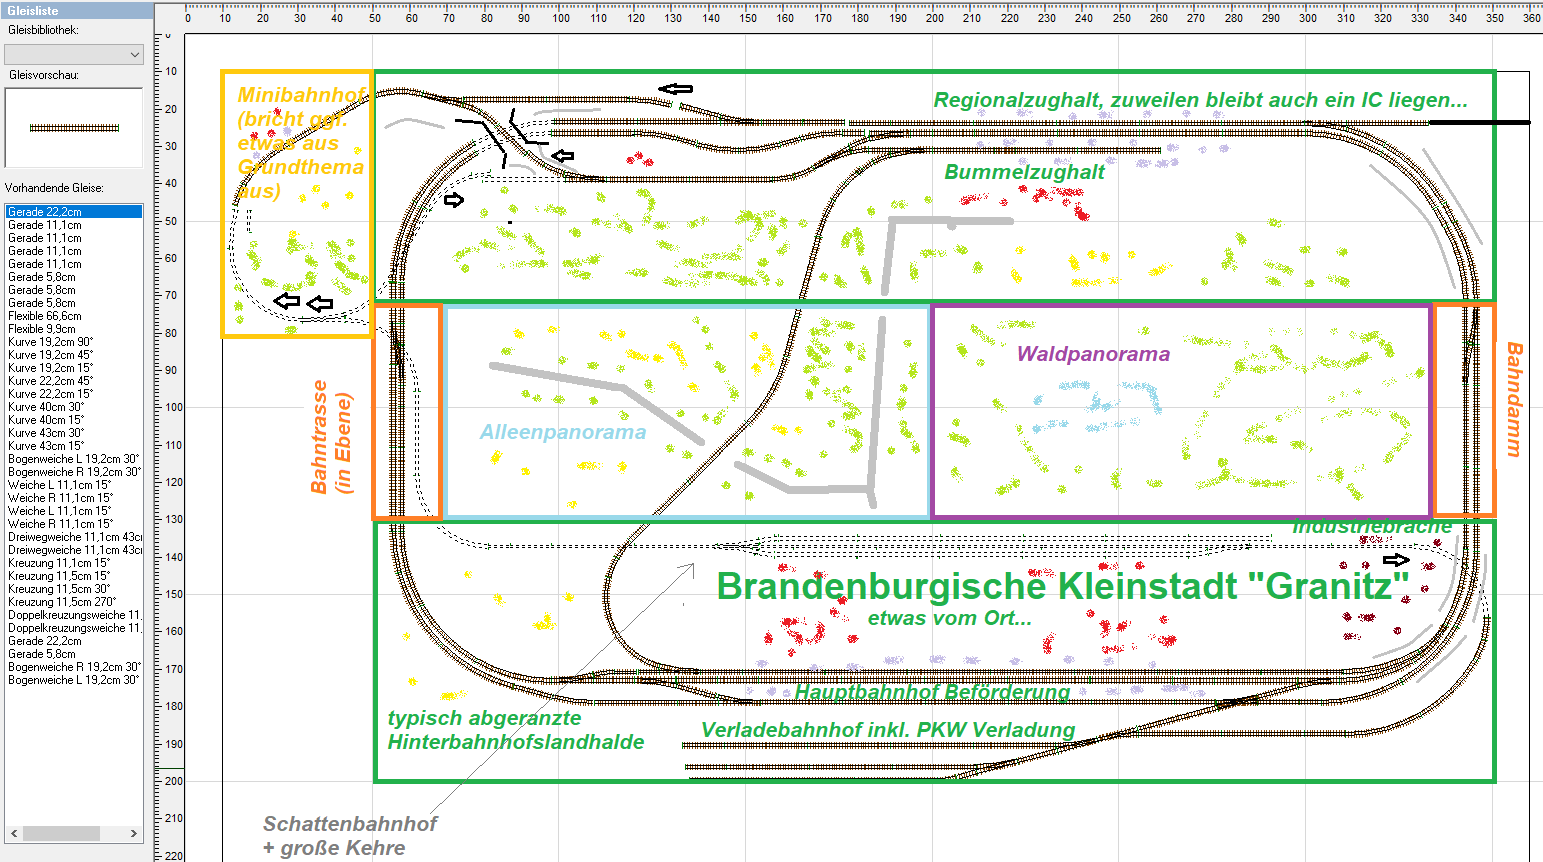
\includegraphics[width=1.0\textwidth]{img/map_evolution/state0-1_granitz_modules_details.png}
   \caption{Urspr\"ungliche Planung f\"ur Vollausbau}
    \label{img:state0-1_granitz_modules_details}
    \end{subfigure}
		\vspace{0.5cm}
	\begin{subfigure}[b]{1.0\textwidth}
    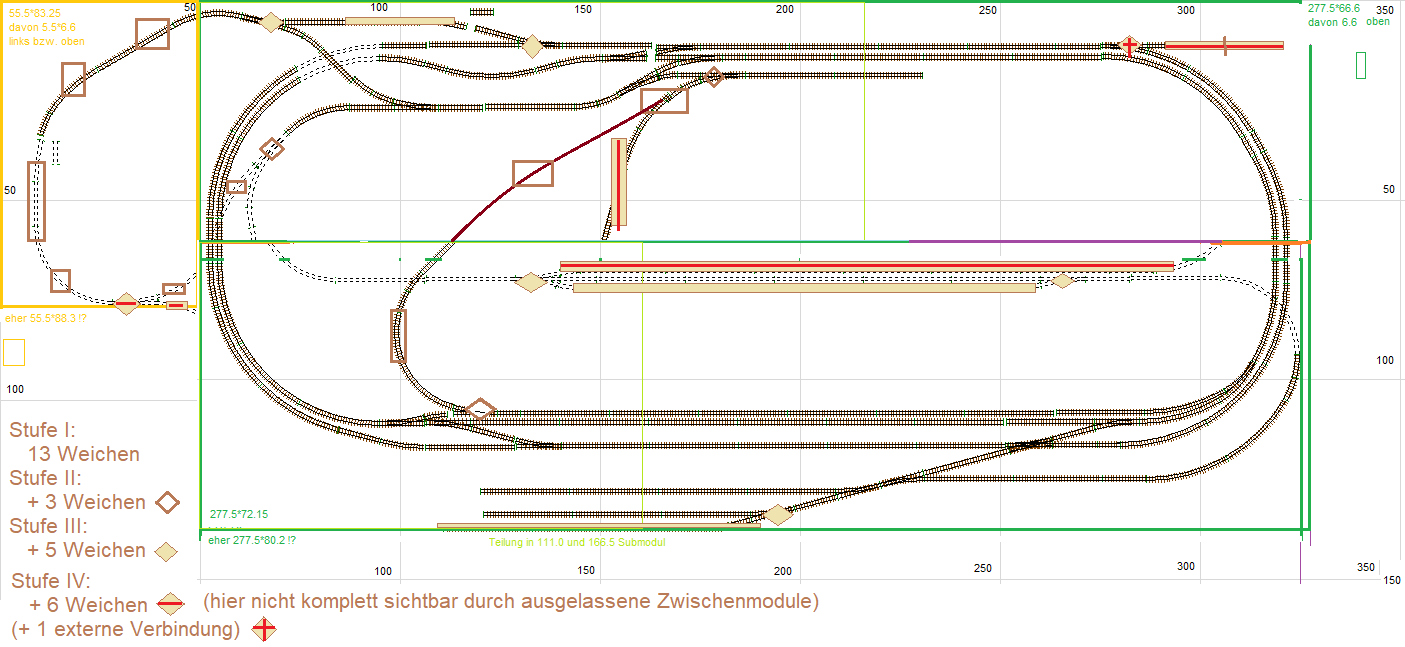
\includegraphics[width=1.0\textwidth]{img/map_evolution/state0-1_granitz_modules_compressed.png}
   \caption{Komprimierte Anlage f\"ur fr\"uhe Ausbaustadien}
    \label{img:state0-1_granitz_modules_compressed}
    \end{subfigure}
	\caption{Erste Entwurfsserie, ausgef\"uhrt als segmentierte Rechteckanlage}
	\label{img:state0-1_granitz}
\end{figure}

\clearpage

Die zentralen Panoramasegmente sowie das Segment der Stadt Granitz selbst sind aus Abb.~\ref{img:state0-1_granitz_modules_details} heraus selbsterkl\"arend.
Der Schattenbahnhof hat allein die Funktion von Abstellgleisen und einer gro{\ss}en Wendeschleife, die zwischen Nordwest und S\"udost befahren werden kann.
Allein ein Merkmal soll hier explizit aufgef\"uhrt werden, das f\"ur alle Entwurfsphasen mandatorisch war und ist:
\begin{itemize}
	\item Bahnsteige m\"ussen eine Kapazit\"at von mindestens f\"unf (Fernverkehr) bzw. vier  (Regionalverkehr) Personenwagen aufweisen.
	Dies gibt somit die Bahnsteigl\"angen in Granitz sowie am Regionalhalt vor.
	\item Eine Kapazit\"at von sechs Personenwagen in Granitz ist dar\"uber hinaus ausdr\"ucklich angestrebt.
\end{itemize}

Modelleisenbahnanlagenbau kann viel Zeit in Anspruch nehmen.
F\"ur mich war und ist es wichtig, bald schon mal einen Zug fahren lassen zu k\"onnen.
Zusammen mit den bereits angedeuteten Problemen bzgl. Platzmangels in der Wohnung wurde schon sehr fr\"uh die Modularisierung in Segmente auf den Plan gesetzt.
Insbesondere 2018 erschien es als absolut unrealistisch, eine Plattentiefe von $2m$ in der Wohnung zu realisieren.
Als Kombil\"osung beide Aspekte betreffend wurde die komplette Entnahme des mittleren Segmentriegels als Option geplant, s. Abb.~\ref{img:state0-1_granitz_modules_compressed}.

Dies erfordert f\"ur eine Anpassung der (urspr\"unglichen) finalen Anlage gem\"a{\ss} Abb.~\ref{img:state0-1_granitz_modules_details} wenig \"Anderungen an der Gleisf\"uhrung:
\begin{enumerate}
	\item Die Nebenstrecke braucht eine alternative, flachere Zuf\"uhrung zum Regionalhalt.
	Dies kann auch bei einem m\"oglichen Hin- und Herwechseln zwischen der komprimierten und Vollvariante bestehen bleiben, indem \"uber eine zus\"atzliche, am Westausgang vom Bummelzughalt einzubauende Weiche (hier nicht abgebildet) jeweils das nicht genutzt Gleis als Totgleis definiert wird.
	\item Der westliche Schleifenschluss in der Schattenbahnhofsebene erfordert eine geringf\"ugige Anpassung.
\end{enumerate}
Es sei darauf verwiesen, dass der mittlere Segmentriegel mit eine Tiefe von $55.5~cm$ bemessen wurde, dementsprechend auf Standardl\"angen vom verwendeten Gleismaterial ausgelegt wurde.

Als zus\"atzliche Information enth\"alt Abb.~\ref{img:state0-1_granitz_modules_compressed} verschiedene Baulose f\"ur den Bastler.
Diese waren sowohl in zeitlich und gestalterisch sinnvolle Abschnitte unterteilt als auch in Budgetierungsabschnitte, um den geringen Gleisbestand aus der Kinderanlage haushaltspolitisch vertr\"aglich zu erweitern.

Letztendlich entsprechen diese Erstentw\"urfe dem klassischen Oval mit etwas Nebenstreckenfirlefans.
Das war dem Autor fr\"uh bewusst aber auch okay so.
Es ging darum, mal einen Zug fahren zu lassen, etwas \"uber die Nebenstrecken und mit dem Schattenbahnhof zu variieren und sich vor allem an den beiden Panoramaplatten gestalterisch auszutoben.
Siehe hierzu auch die in der Einleitung beschriebene Geisterung f\"ur Brandenburg und das ganze drum herum.
Die Fahrstrecke zwischen Granitz und dem Regionalhalt war mit ca. $3m$ (\"uber Granitz-West) bzw. ca. $2m$ (\"uber Granitz-Ost) auch annehmbar.


\subsubsection{Wage Ann\"aherung an den Hundeknochen \"uber die Abgeknickte Acht}
\label{sec:map_development_state2}

Der Entschluss einer tats\"achlichen Umsetzung der Anlage konnte aus Platzgr\"unden nur durch eine konstruktive, ggf. radikale Abwandlung erfolgen.
Wie bereits erw\"ahnt, hat mir der Input von \cite{Gee17} ungemein dabei geholfen, den Prozess geistig in Gang zu setzen.

Der offensichtlichste Nachteil des Ovalkonzepts blieb die Klobigkeit.
Eine Tiefe von $2~m$ verhindert zwangsl\"aufig die Aufstellung an der Wand, da es fr\"uher oder sp\"ater zu Entgleisungen etc. kommen muss.
Der zus\"atzlich einzuplanende und vor allem freizuhaltende Durchgangsbereich macht ein Raumkonzept schnell zunichte.
In dem Raum, wo Granitz nun aufgebaut wird, stand vormals ein Kickertisch, der schon viel Platz in Beschlag genommen hat, aber eine Korpustiefe von $75~cm$.

Gleichzeitig ist das pure Oval nat\"urlich auch nicht besonders attraktiv.
Eine Auffaltung des Anlagenkonzepts bietet demgegen\"uber neue Optionen unter der Voraussetzung, selbst unter der Anname, dass die Grundfl\"ache der Anlage konstant bleibt:
\begin{itemize}
	\item Die Fahrstrecke wird automatisch verl\"angert.
	Ein Beispiel hierf\"ur sei das Umarrangieren des Ovals zu einer Banane oder Umfalten zu einer abgeknickten Acht:
	\begin{itemize}
		\item Die weniger tiefen Segmente in L-Anordnung erfordern mehr Strecke, da der Weg sinnbildlich zur\"uckgefahren werden muss.
		\item Die l\"angere Strecke resultiert zugleich in einer l\"angeren und somit etwas realistischeren Fahrzeit zwischen den Bahnh\"ofen.
		\item Eine Option ist, die zus\"atzliche Strecke ebenfalls in die Ebene 0 zu legen.
		F\"ur ein Brandenburger Thema geht dabei viel Platz f\"ur das Diorama verloren (gro{\ss}er Nachteil).
		F\"ur ein Thema im Mittelgebirge oder Voralpenland ist dies \"uber Tunnels auffangbar.
		\item Die zweite Option ist, die zus\"atzliche Strecke in die Schattenbahnhofsebene zu verlegen.
		Das wurde hier gemacht.
		Ein Nachteil ist, dass dadurch auch potenzielle Panoramastrecke verlorengeht bzw. der Zug die meiste Zeit unsichtbar ist.
		Dieser Nachteil besteht beim normalen Tunnel aber ebenfalls und ist allgemeinhin aus Autorensicht ein absolut gangbarer Kompromiss.
	\end{itemize}
	\item Ein ganz erheblicher Mehrwert ist der Aspekt des Betrachterwinkels, der ebenfalls in \cite{Gee17} thematisiert wird:
	\begin{itemize}
		\item Der Blickbereich eines Betrachters liegt, direkt am Anlagenrand stehend, ca. $1~m$.
		Ein gr\"o{\ss}erer Abstand ist vor allem dann nicht sinnvoll, wenn es um die Detailbetrachtung des Dioramas geht.
		\item F\"ur die Beobachtung von Z\"ugen in Panoramastrecken sch\"atze ich ca. $1.5~m$ als realistisch ein.
		L\"angere Panoramastrecken erfordern zwangsl\"aufig die Bewegung des Beobachters (zumindest mit dem Kopf).
		\item Der letzter Punkt ist entscheidend: Die Bewegung des Beobachters erlaubt die \"Uberf\"uhrung in ein neues Panorama.
		\item Im Umkehrschluss muss ein individuelles Panorama aber auch eine gewisse Mindestbreite aufweisen.
		\item Die L- und U-Form sind f\"ur einen Panoramawechsel noch geeigneter, da sie eine Drehung des Beobachters erfordern und ihn somit zu einer viel markanteren Blickwinkelverlagerung zwingen (ebenfalls sinngem\"a{\ss} von \cite{Gee17} entnommen).
	\end{itemize}
\end{itemize}

Das Ergebnis der Auffaltung in die abknickte Acht ist in Abb.~\ref{img:state2_granitz_modules_details} (ohne Schattenbahnhof aus Gr\"unden der \"Ubersichtlichkeit) sichtbar:
\begin{itemize}
	\item Sch\"onblick befindet sich nun im Nordosten der Anlage
	\item Die Westausfahrt von Granitz f\"uhrt nun \"uber die Schattenbahnhofsebene zum Regionalhalt (inzwischen in Granitz-Walddort umgewidmet)
	\item Der Regionalhalt selbst befindet sich auf dem k\"urzeren L-Schenkel
	\item Die Ostausfahrt von Granitz f\"uhrt \"uber einen kurzen, unter Sch\"onblick verborgenen Bogen in die Gleisgabelung, die in den Erstentw\"urfen von Abb.~\ref{img:state0-1_granitz} noch oben lag
	\item Es ist deutlich sichtbar, dass die Gleisgabelung nun vom Regionalhalt separiert ist, verbunden \"uber die gro{\ss}e Kehrkurve im S\"udosten
\end{itemize}

Es ist au{\ss}erdem eine optionale, zweigleisige Ausf\"adelung zu einem m\"oglichen Zusatzsegment vorgesehen.
Dieses w\"urde letztendlich in einer U-Form resultieren.

\begin{figure}[h]
\centering
  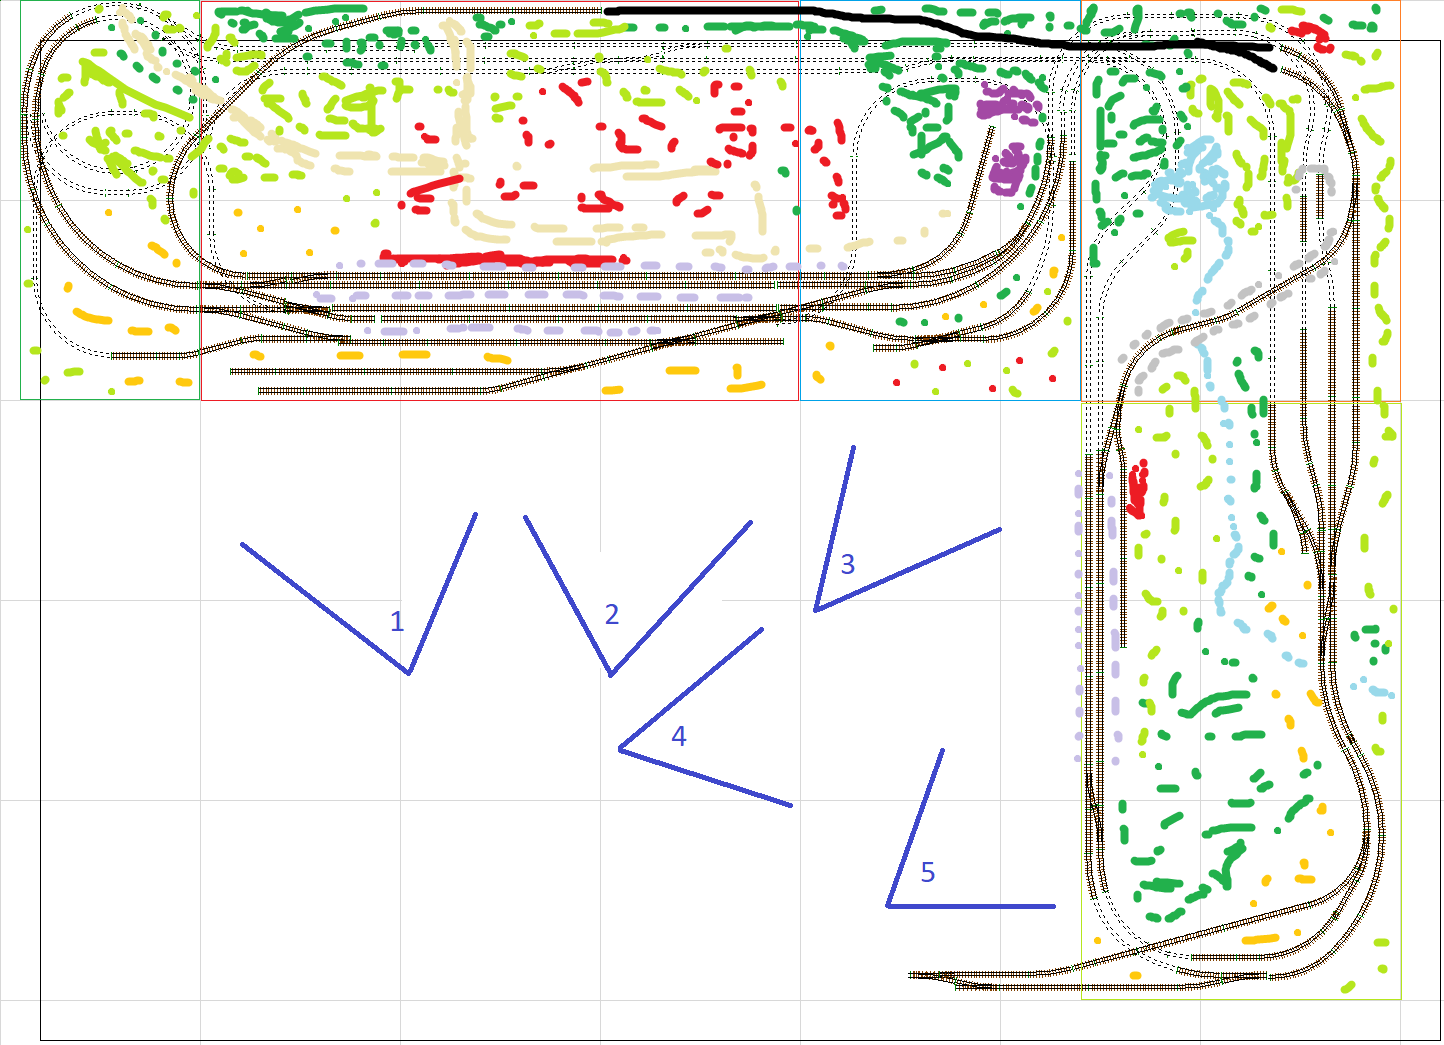
\includegraphics[width=1.0\textwidth]{img/map_evolution/state2_granitz_modules_details.png}
	\caption{Abgeknickte Acht mit flexiblerer Einbindung des Schattenbahnhofs}
	\label{img:state2_granitz_modules_details}
\end{figure}

In der Tat geht nun durch die Trennung von Regionalhalt und Gleisgabel sowie die neue Nebenstreckenf\"uhrung Platz f\"ur die szenische Ausgestaltung verloren.
Auf der anderen Seite ergeben sich neue M\"oglichkeiten - nicht zuletzt auch eine etwas l\"angere Panoramstrecke f\"ur die Nebenstrecke.

\clearpage

Dieses Konzept hat tats\"achlich schon viel von der finalen Umsetzung.
De facto ist es nach wie vor ein zur Acht modifiziertes Oval.
Durch die nun aber r\"aumlich viel deutlicher abgetrennten Abzweige in die Schattenbahnhofsebene und angepassten Gleiswechsel, k\"onnen aber auch spannendere Varianten f\"ur Punkt zu Punkt Verbindungen mit dem Schattenbahnhof gefahren werden.
Die grunds\"atzliche Erweiterbarkeit an der Kehrkurve im S\"udosten w\"urde dar\"uber hinaus viel Potenzial bieten, und sei es nur durch einen weiteren Geisterbahnhof.
\begin{itemize}
	\item Der Schattenbahnhof wird ab diesem Stadium als \textbf{Schattenwalde} gelistet
	\item Der Schattenbahnhof kann zus\"atzlich auch als fiktives Alternativziel in der Ferne verwendet werden, denn \"Uberf\"uhrungsfahrten sind von Granitz aus jeweils im Osten und Westen m\"oglich sowie nach wie vor einmal an der Gleisgabelung.
\end{itemize}
Zwischenzeitlich war sogar noch eine \"Uberf\"uhrung vom Bahnhof Sch\"onblick geplant.
Diese wurde zum einen wegen des gro{\ss}en zu \"uberwindenden H\"ohenunterschieds und zum anderen im Sinne von too much verworfen.

Die Gesamtl\"ange der Anlage sowie ihre L-Form erm\"oglichen gem\"a{\ss} oben ausgef\"uhrten Punkten nun mehrere Blickwinkel des Betrachters, die auch in Abb.~\ref{img:state2_granitz_modules_details} markiert sind:
\begin{enumerate}
	\item Der Bahnhof von Granitz mit der Westausfahrt, dahinter das Alleenpanorama sowie einen Teil der Stadt
	\item Den Ostbereich des Bahnhofs von Granitz mitsamt der angrenzenden Industriebrache und nach hinten verlagerten Panoramastrecke der Nebenbahn
	\item Das fast ausschlie{\ss}lich durch den Schwenk der Nebenbahn dominierte Diorama von Sch\"onblick samt der nun vorgelagerten Wiese und Teich, seitlich begrenzt durch die R\"uckf\"uhrung der Nebenstrecke in Richtung Regiohalt
	\item Der Regiohalt Granitz-Walddorf, umgeben vom Wald mit Bachlauf
	\item Die S\"udostkehre und der Blick auf die Gleisgabel im Hintergrund
\end{enumerate}

Abschlie{\ss}end zu diesem Konzept sollen die M\"oglichkeiten betrachtet werden, die der Bahnhof Granitz selbst liefert.
Das h\"ochste Verkehrsaufkommen bietet dabei nat\"urlich die Hauptstrecke, die durch Nebengleise auch als Endpunkt f\"ur RB/RE Verbindungen fungieren kann.

Zun\"achst soll nun aber die Philosophie der Nebenstreckenplanung h\"oher aufgel\"ost werden.
Die Nebenstrecken seien grob wie folgt definiert:
\begin{enumerate}
	\item \textbf{Lokale Nebenstrecke:}\\
	Hierbei handelt es sich um die bisher schon behandelte Nebenstrecke, die \textbf{Granitz} \"uber \textbf{Sch\"onblick} mit \textbf{Granitz-Walddorf} verbindet.
	Sie ist nicht elektrifiziert.
	Im Personenverkehr ist sie f\"ur Kurzz\"uge sowie Museumsfahrten vorgesehen.
	Prinzipiell ist sie auf f\"ur den G\"uterverkehr freigegeben zum Zweck von \"Uberf\"uhrungsfahrten auf die Hauptstrecke mit Transitpunkt Gleisgabel.
	\item \textbf{Nebenstrecke Schattenwalde:}\\
	Die Strecke ist elektrifiziert und in die Ostausfahrt aus Granitz integriert.
	Es findet mit der Ausfahrt eine \"Uberf\"uhrung in die Schattenbahnhofebene statt.
	Im Personenverkehr kann sie beliebige Regionalz\"uge, im G\"uterverkehr beliebige Zuggarnituren bedienen.
	\item \textbf{Nebenstrecke westliche D\"orfer:}\\
	Es handelt sich um eine nicht elektrifizierte, tendenziell stillgelegte Nebenstrecke.
	Die Ausfahrt ist im westlichen G\"uterbahnhofsbereich von Granitz verzeichnet, hier noch als \"Uberf\"uhrung zum Schattenbahnhof.
	Letzteres Konzept wurde nachfolgend aus Gr\"unden der Komplexit\"at verworfen.
	Es bleibt alternativ die Andeutung als Gleis am linksunteren Plattenende und somit m\"oglichen Anschlusspunkt f\"ur weitere, westlich anflanschbare Segmente.
	\item \textbf{Industrienebenstrecke:}\\
	Hierbei handelt es sich um den kurzen Abzweig am Ostende des stadtseitigen Personengleises im Bahnhof von Granitz, der auf das Fabrikgel\"ander einsticht.
	Mit einer weiteren Weiche wird diese Strecke ggf. geradeaus bis an den n\"ordlichen Segmentrand verl\"angert und w\"urde dann auch eine Unterf\"uhrung der lokalen Nebenstrecke erfordern.
	Sicher ist in jedem Fall, dass zu keinem Zeitpunkt die Streckenf\"uhrung \"uber das Fabrikgel\"ande hinaus in Betrieb ist:
	Diese Nebenstrecke ist definitiv stillgelegt und \"Uberwucherung ist deutlich erkennbar.
\end{enumerate}

Die Gleise im Bahnhof von Granitz seien durchnummeriert von Norden (oben) nach S\"uden (unten):
\begin{itemize}
	\item[I] Personenverkehr
	\begin{itemize}
		\item Erster Bahnsteig, direkt am Empfangsgeb\"aude
		\item Bedienung Hauptstrecke und lokale Nebenstrecke
		\item Regul\"are Kapazit\"at: 6 Personenwagen + Lok
		\item Erweiterbare auf: 7 Personenwagen + Lok
		\item Es bleibt eine direkte Versorgung des anschlie{\ss}enden, im sp\"ateren Verlauf auf der Zeitschiene stillgelegten Fabrikgel\"andes m\"oglich.
	\end{itemize}
	\item[II] Personenverkehr und allgemeiner Durchfahrtsverkehr
	\begin{itemize}
		\item Zweiter Bahnsteig
		\item Bedienung der Hauptstrecke
		\item Kapazit\"at: 5 Personenwagen + Lok oder 6 Personenwagen mit z.T. vorgelagerter Lok
	\end{itemize}
	\item[III] Personenverkehr und allgemeiner Durchfahrtsverkehr
	\begin{itemize}
		\item Zweiter Bahnsteig, s. Gleis II
	\end{itemize}
	\item[IV] Personenverkehr
	\begin{itemize}
		\item Dritter Bahnsteig
		\item Bedienung der Hauptstrecke von Westen her mit Endpunkt Granitz
		\item Kapazit\"at: 4 Personenwagen + Lok
		\item Lokomotivumstellung \"uber Gleis V durchf\"uhrbar
	\end{itemize}
	\item[V] Personenverkehr und G\"uterverkehr (Durchfahrt, Zwischenrangierung)
	\begin{itemize}
		\item Dritter Bahnsteig
		\item Bedienung der Nebenstrecke Schattenwalde und ggf. Hauptstrecke von Osten her mit Endpunkt Granitz
		\item Kapazit\"at: 4 Personenwagen + Lok
		\item Lokomotivumstellung \"uber Gleis IV durchf\"uhrbar, alternativ in angepasstem Szenario auch \"uber Gleis VI
	\end{itemize}
	\item[VI] G\"uterverkehr
	\begin{itemize}
		\item Allgemeiner G\"uterverkehr
		\item Direkte Zufuhr von Osteinfahrt, Gleis II
		\item Abfuhr Ostausfahrt nur \"uber Verl\"angerung Gleis IV mit sp\"aterem Wechsel auf Gleis III im verdeckten Gleisbogen
		\item Zu- und Abfuhr nach Westen nur durch Rangieren \"uber Verl\"angerung Gleis IV
	\end{itemize}
	\item[VII] G\"uterverkehr, PKW-Verladung
	\begin{itemize}
		\item Prinzipiell analog zu Gleis VI
	\end{itemize}
\end{itemize}
	
Die Rationalisierung einiger \"Uberf\"uhrungen in die Schattenbahnhofsebene erfolgte prim\"ar durch erforderte Steigungen, die f\"ur den Modelleisenbahnbetrieb nicht durchf\"uhrbar sind.
F\"ur die Westausfahrt von Granitz wurde hier erstmalig der Bau einer Gleiswendel um ca. $450^{\circ}$ als notwendig erachtet.



\subsubsection{Ann\"aherung an das Eigentliche Punkt zu Punkt Konzept}
\label{sec:map_development_state3}

Eine Abwandlung des Gleisplans stellt der Stand von Abb.~\ref{img:state3_granitz_modules} dar.
Die relativ kleine, aber entscheidende Hauptma{\ss}nahme ist im nun eingezeichneten U- bzw. J-Schenkel-Segment zu sehen.
Dieses wird genutzt, um die beiden getrennten Panoramastrecken bei Granitz-Walddorf sowie der Gleisgabelung realistischer auslaufen zu lassen.
Dies erfolgt durch die Aufgabe der Kehrkurve.
Vielmehr k\"onnen beide Strecken nun mit gr\"o{\ss}eren Initialradien auf das neue S\"udsegment abgeleitet werden.

\begin{figure}[h]
\centering
  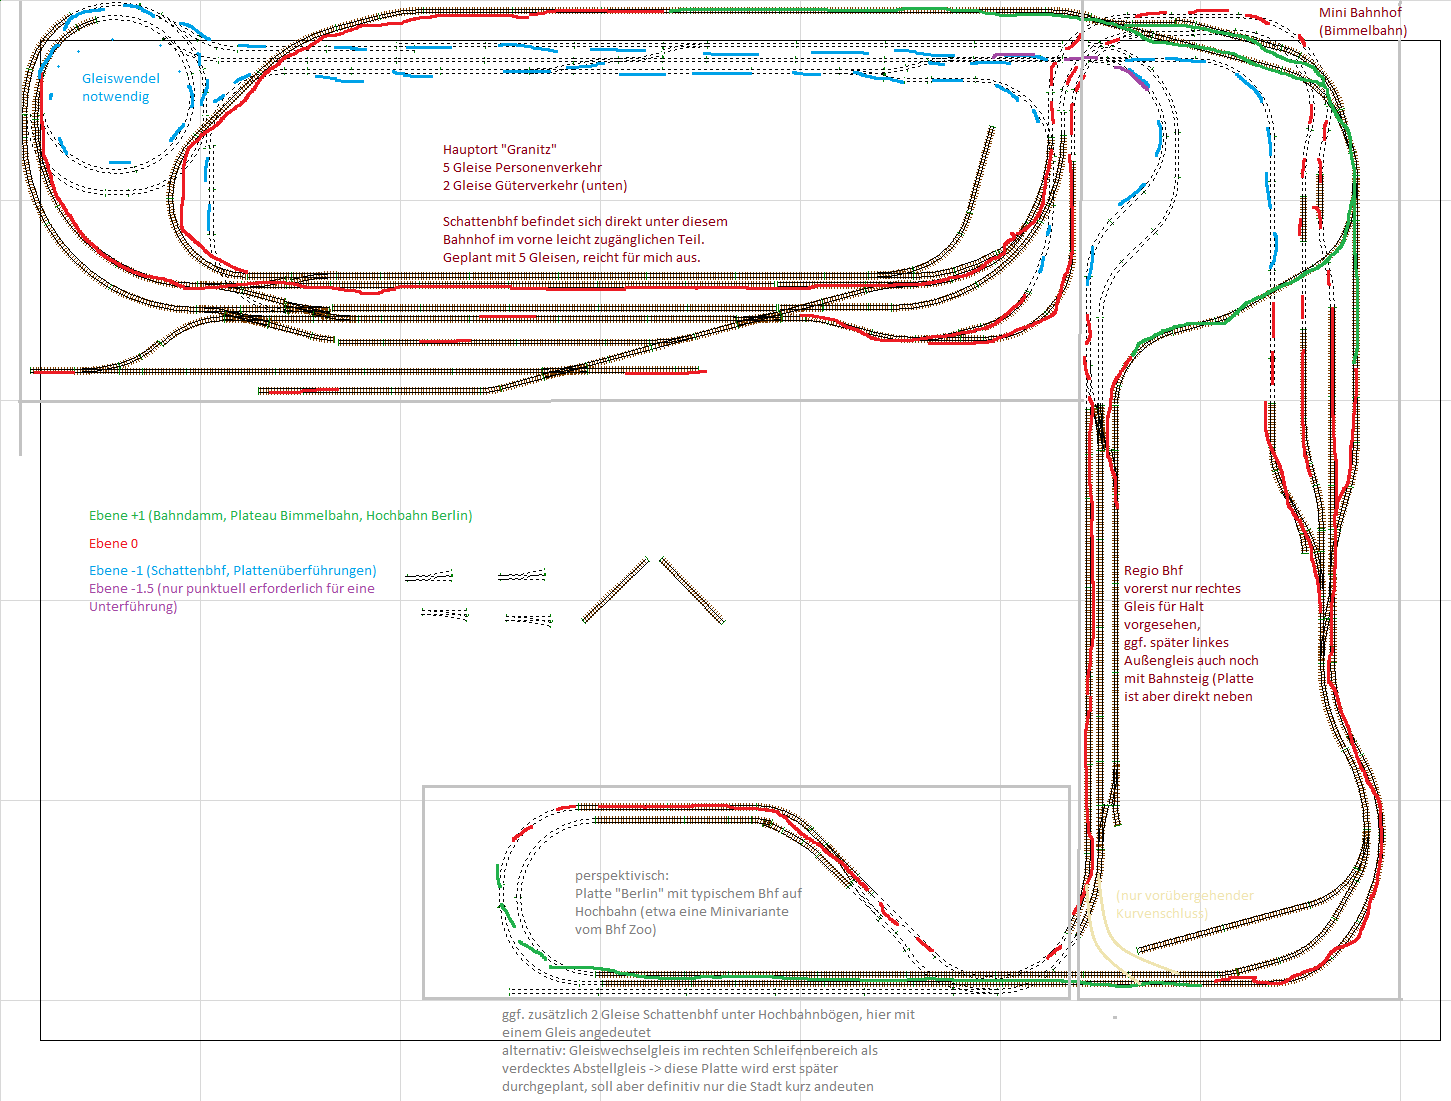
\includegraphics[width=1.0\textwidth]{img/map_evolution/state3_granitz_modules.png}
	\caption{Option zur Punkt zu Punkt Erweiterung durch Segmentierung in J-Form}
	\label{img:state3_granitz_modules}
\end{figure}

Die Ausgestaltung des S\"udsegments ist an dieser Stelle nicht entscheidend.
Verschiedene M\"oglichkeiten k\"onnen vorgesehen werden, so z.B.
\begin{itemize}
	\item wie abgebildet:
	W\"ahrend die Trasse von Granitz-Walddorf zun\"achst verdeckt gef\"uhrt wird, dann vorgelagert und in einer halben Gleiswendel m\"undet, wird die Trasse von der Gleisgabelung aus bereits auf dem Ostsegment auf eine h\"ohere Ebene verlagert und endet auf dem S\"udsegment in einem weiteren Bahnhof oder eine Panoramastrecke.
	\item operative Trennung beider Bahntrassen:
	Die Trassen erhalten verdeckt oder z.T. sichtbar Endbahnh\"ofe, so dass ein echtes Punkt zu Punkt Konzept entsteht.
	\item operative Trennung, aber mit optionaler Verbindungskehre zum Showbetrieb:
	Dieses Konzept entspricht im Prinzip dem zuvor beschriebenen, aber beh\"alt die bereits in der Abbildung angedeutete Gleiswende zumindest eingleisig bei.
	Dies erfolgt dann nur f\"ur eine noch gr\"o{\ss}ere Erweiterbarkeit der operativen M\"oglichkeiten oder der Change f\"ur einen durchgehenden Acht-Betrieb mit z.B. Kindern.
	Dieses Konzept wird nachfolgend in Kap.~\ref{sec:map_date} als aktueller Variante kurz dargestellt.
\end{itemize}
F\"ur fr\"uhe Bauphasen oder auch nur einen tempor\"aren Aufbau des S\"udsegments besteht weiterhin die M\"oglichkeit, die Kehrkurve auf dem Ostsegment durch wenige Eingriffe wiederherzustellen.
Dieser Punkt ist auch insofern wichtig, als dass mit dem Ausbau zur U-Form nun doch wieder erhebliche Zweifel am verf\"ugbaren Platz im Wohnraum aufkommen...

Ein paar kurze Worte seien noch zu sekund\"aren Modifikationen genannt:
\begin{enumerate}
	\item Die Gleise IV und VI sind \"uber die angedeutete \"Uberf\"uhrung in die stillgelegte \textbf{Nebenstrecke westliche D\"orfer} miteinander verbunden.
	Dies erm\"oglicht einen besseren Rangierbetrieb f\"ur die den St\"uckgutverkehr abwickelnden Lokomotiven.
	\item Der Bahnhof Granitz-Walddorf - zuvor f\"ur den Personenverkehr \"uber alle drei Gleise ausgelegt - ist nun auf ein bedienbares Gleis reduziert.
	Dies entspricht so manchem Vorbild von Regionalhalten in Brandenburg - gro{\ss}er Dank geht an dieser Stelle an meinen Bruder f\"ur die Idee.
	Eine Ausr\"ustung des anderen Au{\ss}engleises bleibt dennoch m\"oglicht und w\"urde das mittlere Gleis f\"ur Durchfahrten beibehalten.
	\item Ebenfalls den Bahnhof Granitz-Walddorf betreffend ist die nun beidseitige \"Uberf\"uhrungsm\"oglichkeit auf die Hauptstrecke.
	Diese wurde mit der zuvor beschriebenen Ma{\ss}nahme erforderlich.
	Zuvor endete das Gleis der \textbf{lokalen Nebenstrecke} im Bahnhof.
\end{enumerate}

Abschlie{\ss}end zeigt Abb.~\ref{img:state3_granitz_modules} eine Einf\"arbung der verschiedenen Ebenen:
\begin{itemize}
	\item Rot: Ebene 0
	\item Gr\"un: Ebene +1 (maximal $+10~cm$)
	\item Blau: Ebene -1, Schattenbahnhof (Schattenwald ca. $-15~cm$, \"Uberf\"uhrungstrasse von Granitz-West nach Granitz-Walddorf ca. $-10~cm$
	\item Gestrichelt: Allgemein verdeckter Bereich, unabh\"angig von Ebene
\end{itemize}
Es sei angemerkt, dass der Schattenbahnhof selbst wiederum nicht vollst\"andig in der Abbildung ausgef\"uhrt ist.
Allgemein befindet er sich unterhalb vom Bahnhof Granitz, einfach von der Vorderkante des Nordsegments zugreifbar.
Die hier dargestellte Version sieht den Schattenbahnhof als Kopfbahnhof vor, dessen Einfahrt unter der Westeinfahrt von Granitz Bahnhof liegt.





\subsection{Aktueller Gleisplan}
\label{sec:map_date}

Figure~\ref{img:stateDate_granitz_modules} zeigt den aktuellen Planungsstand.

\begin{figure}[h]
\centering
  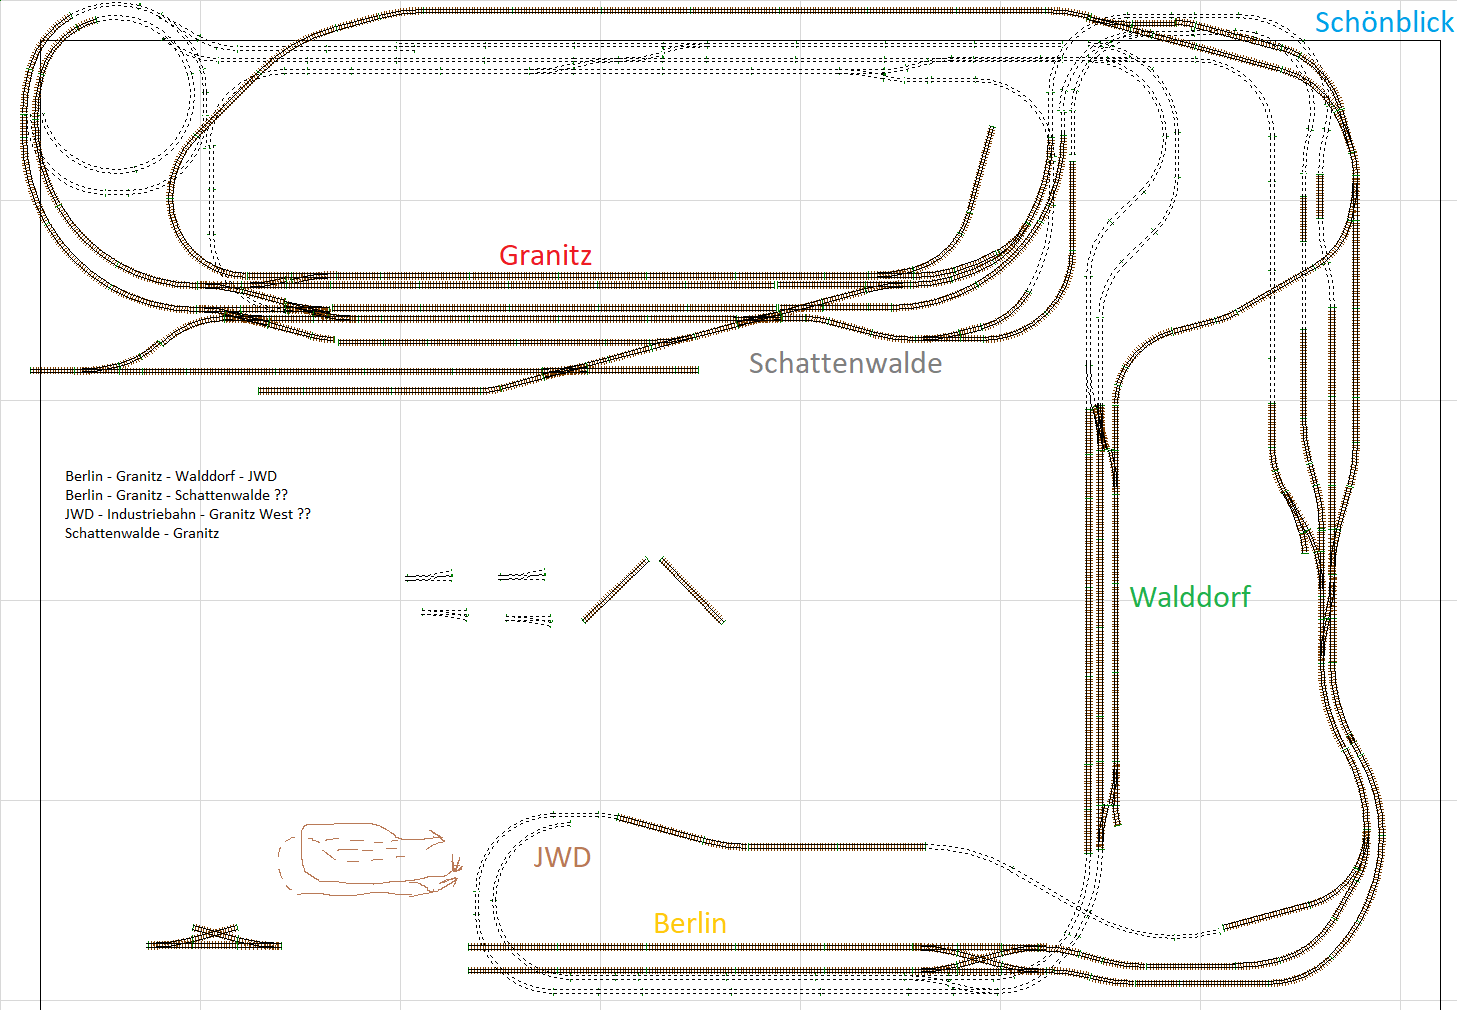
\includegraphics[width=1.0\textwidth]{img/map_evolution/stateDate_granitz_modules.png}
	\caption{Aktueller Planungsstand, auszuf\"uhren durch Segmentierung in J-Form}
	\label{img:stateDate_granitz_modules}
\end{figure}

Der wesentliche Unterschied zum Stand in Kap.~\ref{sec:map_development_state3} besteht in der bereits diskutierten Alternativausf\"uhrung vom S\"udsegment.
\begin{itemize}
	\item Endpunkt der Trasse von Granitz-Walddorf kommend ist ein kleiner Schattenbahnhof genannt \textit{JWD} (Janz weit drau{\ss}en)
	\footnote{\textit{JWD} entspringt dem Berliner und Brandenburger Jargon und bezeichnet zun\"achst alles, was weit ab vom Schuss bezeichnet.
	Von Berlin ausgesehen muss man Granitz selbst als JWD bezeichnen.
	Hier meint es aber - ausgehend von Granitz als Zentrum der Modellbahnwelt - beliebige Regional- und Fernverkehrsziele.}.
	JWD ist hier das ultimative Synonym f\"ur beliebige Ziele, die fiktiv jenseits der Modellbahnanlage sind.
	\item Endpuntk der Trasse von der Gleisgabel kommend ist ein Hochbahnhof.
	Dieser k\"onnte z.B. an den Berliner Bahnhof Zoologischer Garten angelehnt sein.
	Aus diesem Grund wird das S\"udsegment sicherlich auch in nachfolgenden immer wieder als \textbf{Berlin} bezeichnet werden.
\end{itemize}

Der ultimative Knackpunkt im f\"ur den finalen Ausbaustand anvisierten Konzept ist aber die Kehre im S\"udsegment.
Diese verbindet nun letztlich den Schattenbahnhof JWD eingleisig mit einer neuen Nebenstrecke, welche s\"udlich von der Gleisgabelung in die Hauptstrecke aufgeht.
Die szenische Ausgestaltung ist noch nicht fixiert.
Zwei Optionen werden gehandelt:
\begin{enumerate}
	\item Bahnschneise in Berlin (in dieser Form als ziemlich un\"ublich angesehen)
	\item Dioramatechnisch vom Bahnhof abgehobene Industrienebenstrecke in oder bei Berlin (der Cut in der Szenerie ist hier der Nachteil)
\end{enumerate}
Eine totale Verdeckung ist ebenfalls denkbar, w\"are aber schade.
Gerade hier bietet sich die M\"oglichkeit einer weiteren Panoramafahrt.

Allgemeinhin soll diese neue Nebenstrecke aber dem G\"uterverkehr vorbehalten sein.

F\"ur das S\"udsegment wurden insbesondere hinsichtlich der Lage des potenziellen Hochbahnhofs verschiedenste Varianten skizziert.
Da nach wie vor die Bahnsteigkapazit\"aten von mindestens, eher mehr als f\"unf Personenwagen bestehen, ist die Segmentl\"ange entsprechend zu w\"ahlen.
Kompromisse sind nicht m\"oglich, da wir hier immer noch von Berlin sprechend, das keine niedrigere Kapazit\"at als Granitz haben kann!
Zugleich offenbart sich, wie schon in Kap.~\ref{sec:map_development_state3} beschrieben, hier ein praktisches Problem:
Die Begrenzung des f\"ur die Anlage nutzbaren Raums.




\subsection{Projektierter Endausbau}
\label{sec:map_final_projected}

Eine konkrete Endausbaustufe wird hier nicht vorgestellt.
Es existieren aber folgende Grundideen:
\begin{enumerate}
	\item Ausnutzung der Minus 1 Ebenenvom Ost- und ggf. S\"udsegment f\"ur Nebenstrecken, insbesondere Dioramabildung.\\
	$\rightarrow$ nach Abschluss des aktuellen Planungsstands prinzipiell jeder Zeit zumindest f\"ur das Ostsegment realisierbar
	\item Erweiterung des Rangierbereichs vom G\"uterbahnhof Granitz durch Anschluss eines Segments an Granitz-West.
	Dieser w\"urde dann den nicht mehr bewirtschafteten \"Ubergang zur \textbf{Nebenstrecke westliche D\"orfer} andeuten.\\
	$\rightarrow$ als weites Fernziel realisierbar, da hier aktuell ein selbstgebautes, gro{\ss}fl\"achiges Regal anschlie{\ss}t, von dem entsprechend ein Fach ger\"aumt werden m\"usste
	\item Reaktivierung der \textbf{Nebenstrecke westliche D\"orfer} durch Anschluss eines Segments an Granitz-West.
	Analog zu vorherigem Konzept, aber mit weniger Rangierfl\"ache, daf\"ur einer weiteren Gleiswendel, welche letztendlich Erweiterungen in einer weit \"uber Granitz gelagerten Ebene (Minimum: $70~cm$) erm\"oglichen w\"urde.\\
	$\rightarrow$ unrealistisch
	\item Nutzung des S\"udsegments f\"ur eine Gleiswendel analog zu vorherigem Konzept.
	Diese Wendel w\"urde ebenfalls eine nun neue Nebenstrecke auf einer deutlich \"uber dem Ostsegment gelagerten Ebene erlauben.\\
	$\rightarrow$ unrealistisch, da bereits das S\"udsegment mit gro{\ss}er Sicherheit nicht dauerhaft platziert werden kann
	\item Alternative Ausf\"uhrung der \textbf{Nebenstrecke westliche D\"orfer} \"uber einen nahezu O-Schluss der Segmente.
	Dies erm\"oglicht auch noch verh\"altnism\"a{\ss}ig viel L\"ange f\"ur diese Nebenstrecke.\\
	$\rightarrow$ unrealistisch, da noch mehr Platzbedarf von N\"oten und daher wenn \"uberhaupt nur in sauberer Modulbauweise umsetzbar
\end{enumerate}

%\begin{figure}[h]
%\centering
	%\begin{subfigure}[b]{0.49\textwidth}
    %\includegraphics[width=1.0\textwidth]{sub/concept_studies/img/carpets/benefit_maps/map_benefit_s500.png}
   %\caption{$s = 500 NM$}
    %\label{img:carpets_benefit_maps_s500}
    %\end{subfigure}
	%\begin{subfigure}[b]{0.49\textwidth}
    %\includegraphics[width=1.0\textwidth]{sub/concept_studies/img/carpets/benefit_maps/map_benefit_s1000.png}
   %\caption{$s = 1000 NM$}
    %\label{img:carpets_benefit_maps_s1000}
    %\end{subfigure}
		%\begin{subfigure}[b]{0.49\textwidth}
    %\includegraphics[width=1.0\textwidth]{sub/concept_studies/img/carpets/benefit_maps/map_benefit_s2500.png}
   %\caption{$s = 2500 NM$}
    %\label{img:carpets_benefit_maps_s2500}
    %\end{subfigure}
		%\begin{subfigure}[b]{0.49\textwidth}
    %\includegraphics[width=1.0\textwidth]{sub/concept_studies/img/carpets/benefit_maps/map_benefit_s5000.png}
   %\caption{$s = 5000 NM$}
    %\label{img:carpets_benefit_maps_s5000}
    %\end{subfigure}
	%\caption{Straight map of benefits for PSN supply flow modulation}
	%\label{img:carpets_benefit_maps}
%\end{figure}
	
	\section{Betriebsszenario}
\label{sec:operation}


\subsection{Typische Zugverbindungen}
\label{sec:trainConnections}




\subsection{Zugmaterial}
\label{sec:trainMaterial}


	
	\section{Anlage}
\label{sec:anlage}

\subsection{Segmentplatten}
\label{sec:segments}


\subsection{Gleismaterial}
\label{sec:trackMaterial}


\subsection{Gleiswendel}
\label{sec:trackHelix}

Der H\"ohenunterschied zwischen den Gleisebenen der Bahnho\"ofe Granitz und Schattenwald betr\"agt ca. $16~cm$.
Insbesondere f\"ur die Westausfahrt von Granitz vom schmalen Westsegment aus ist eine einfache Rampe in die $-1$ Ebene aufgrund der hohen Steigung nicht praktikabel.
Somit ergab sich hier erstmalig die Notwendigkeit einer Gleiswendel.

Die Gesamtsituation am Westsegment ist in Abb.~\ref{img:anlage_trackHelix_initialMapSituation} durch den Auszug des Gleisplans zu Beginn der Gleiswendelumsetzung angedeutet.
Das Westsegment hat eine Brei von $45~cm$, in der Abbildung eingerahmt durch den rechten roten Balken, oberen Rasterrand und den angedeuteten roten Strich rechts oben.
Demzufolge ist der Platz f\"ur eine Gleiswendel mit $R1$ am Innen- sowie $R2$ am Au{\ss}engleis bereits nicht ohne weiteres realisierbar.
Als zus\"atzliches Problem an der rechts oberen Ber\"uhrfl\"ache des West- mit dem Zentralsegments kommt der an der Unterseite der Platte angeflanschte Stabilisierungsrahmen hinzu. s.~Abb.~\hl{XX}.
Ohne weitere Ma{\ss}nahmen reicht demzufolge f\"ur die erste Halbwindung nicht allein ein H\"ohenunterschied von ca. $4~cm$ aus, der f\"ur eine einfache Untertunnelung des Plattenbodens selbst n\"otig w\"are.

\begin{figure}[h]
\centering
  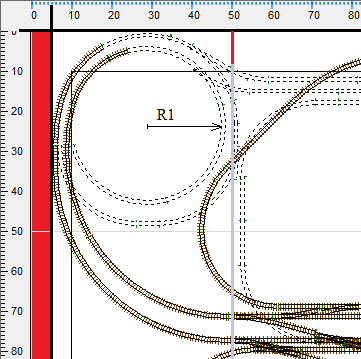
\includegraphics[width=0.35\textwidth]{img/anlage/trackHelix_initialMapSituation.png}
	\caption{Ausgangssituation bei der Planung der Gleiswendel: Westausfahrt von Granitz mit \"Uberf\"uhrung zur Schattenbahnhofsebene}
	\label{img:anlage_trackHelix_initialMapSituation}
\end{figure}

\hl{Lattenrahmen Zentralplatte als Minimap zeigen!}

Angedacht wurde zuerst eine einfache Gleiswendel um ca. $450^\circ$.
Das Innengleis sollte komplett auf $R1$ ausgelegt werden.
F\"ur das Au{\ss}engleis war zumindest in Teilen eine Auslegung mit Flexgleisen geplant.
Die L\"osung der initialen Rahmenunterf\"uhrung wurde zun\"achst aufgeschoben.

Empfehlungen in einschl\"agigen Spur-N Foren nennen Steigungen von $\alpha = \left[ 2 ; 3 \right]^\circ$ als gangbar.
Da dies ganz offensichtlich nicht unter den vorliegenden Randbedingungen eingehalten werden konnte, wurde ein einfacher Testtr\"ager f\"ur die Ermittlung akzeptabler Steigungen erstellt, Abb.~\hl{FIG\_TESTTRAEGER\_STEIGUNG}.
Dieser diente zugleich der Erprobung des h\"aufig angepriesenen Gewindestangenprinzips zur einfachen, flexiblen und gleichzeitig pr\"azisen Justierung der Gleiswendelb\"oden.
Das im Versuchstr\"ager verbaute Gleismaterial war bereits gealtert, um konservativ vorzugehen.
F\"ur die Steigungstests wurde sodann ein Regionalzug verwendet, der als Standard f\"ur das Betriebsszenario von Granitz erachtet wurde.
Die Anzahl der Waggons wurde variiert, um ein Gef\"uhl f\"ur deren Einfluss auf das Verhalten der Lok am Anstieg zu ermitteln.
Insgesamt erschien die Anzahl der Waggons als sekund\"ares Auslegungskriterium.

%25.5 mm

%77 , 77 , 77 mm

%123 mm

Zu den verschiedenen, in Betracht gezogenen Definitionen der Gleiswendel:
\begin{itemize}
	\item Grundlage bildet eine Gleiswendel in Kreis- oder Ovalform.
	\item Bestimmend f\"ur die Auslegung ist das Innengleis mit Verwendung von $R1$ Radien.
	\item Die Radien des Au{\ss}engleises bleiben zun\"achst irrelevant, da gr\"o{\ss}ere Radien bzgl. Steigung unkritischer sind.
	\item Die Fahrwegl\"ange auf einem Viertelkreis ergibt sich somit zu ca. $30~cm$, die eines Halbkreises zu ca. $60~cm$.
	\item Die Ovalisierung der Gleiswendel kann mit beliebigen Standardgr\"o\"{ss}en durchgef\"uhrt werden, im Fall von Arnold N also auf Basis von $5.5~cm$ Geraden, f\"ur alle Steigungsberechnungen konservativ gek\"urzt auf $5~cm$.
\end{itemize}

Mit dem Testtr\"ager ergaben sich Vorergebnisse f\"ur folgende Konfigurationen:
\begin{itemize}
	\item Definition des Versuchstr\"agers:
	\begin{itemize}
		\item Versuchsstrecke Minimum zu Maximum bildet jeweils ein Halboval
		\item Halboval setzt sich zusammen aus $R1 90^\circ$~$\rightarrow$~$22~cm$~\textit{Gerade}~$\rightarrow$~$R1 90^\circ$
		\item Steigung \"uber Gewindestangen justierbar
	\end{itemize}
	\item Standardkonfiguration Testzug: Lok + 3 Doppelstockwagen
	\item H\"ohenunterschied von ca. $2.2~cm$: Gutes Fahrverhalten
	\item H\"ohenunterschied von ca. $5.0~cm$: Noch ausreichendes Fahrverhalten
	\begin{itemize}
		\item Steigung im Versuchstr\"ager: $6.3\%$
		\item Steigung bei m\"oglicher Verl\"angerung der Geraden auf insgesamt 33~cm: $5.6\%$
	\end{itemize}
	\item Die Steigungen \"uberschreiten deutlich die Empfehlungen aus einschl\"agigen Foren.
	\item Es muss ber\"ucksichtigt werden, dass l\"angere Z\"uge und schlechtere Loks ein schlechteres Verhalten an der Steigung aufweisen werden.
	\item[$\Rightarrow$] \textbf{Ein H\"ohenunterschied von $16~cm$ bei einer Windung von $450^\circ$ ist nicht ausreichend.}
\end{itemize}

Aus diesem Grund wurde nun eine doppeletagige Gleiswendel angestrebt.
Tabelle~\ref{tab:anlage_trackHelix_pre_calc_doubleHelix} zeigt hierf\"ur Vorkalkulationen f\"ur resultierende Steigungen.

\begin{table}[h]
	\centering
		\begin{tabular}{lccc}
			H\"ohenunterschied $(cm)$ & Windungen/Etagen $(-)$ & Geradenl\"ange Halboval $(cm)$ & Resultat $\alpha$ $(\%)$ \\
			\hline
			17 & 2 & 20 & 5.3 \\
			17 & 2 & 30 & 4.7 \\
			15 & 2 & 20 & 4.7 \\
			15 & 2 & 25 & 4.5 \\
			15 & 2 & 30 & 4.2 \\
		\end{tabular}
	\caption{Vorrechnungen doppeletagige, ovale Gleiswendel}
	\label{tab:anlage_trackHelix_pre_calc_doubleHelix}
\end{table}








%\begin{figure}[h]
%\centering
	%\begin{subfigure}[b]{0.49\textwidth}
    %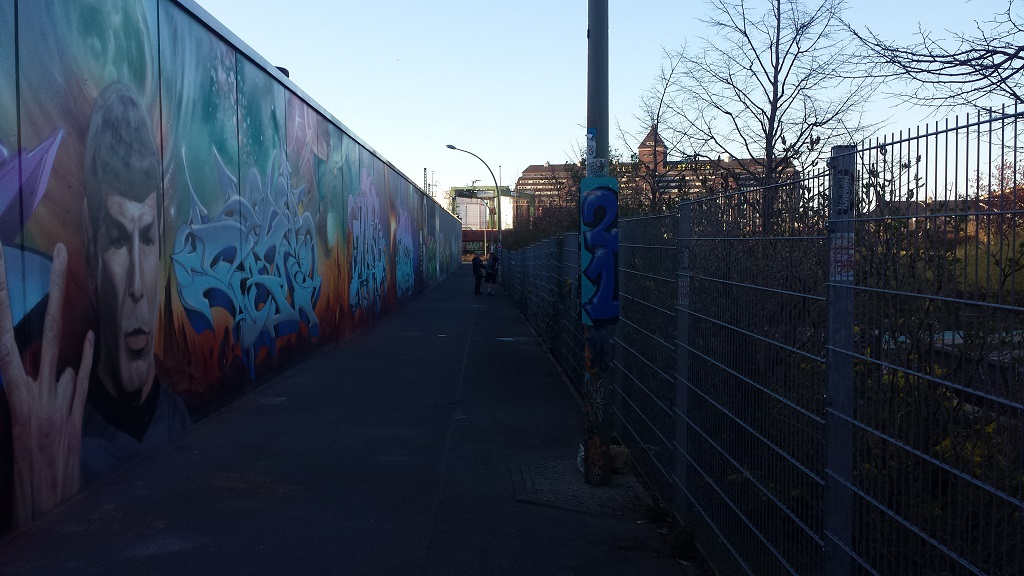
\includegraphics[width=1.0\textwidth]{img/inspiration/westhafen_view_preDurchgang.jpg}
   %\caption{Fu{\ss}g\"angerdurchgang zwischen einem Gro{\ss}handel und dem Stadtgarten am ZK/U, links eine freigegebene Graffitifl\"ache, geradeaus der Westhafen mit vorgelagerter Bahntrasse}
    %\label{img:inspiration_westhafen_view_preDurchgang}
    %\end{subfigure}
	%\begin{subfigure}[b]{0.49\textwidth}
    %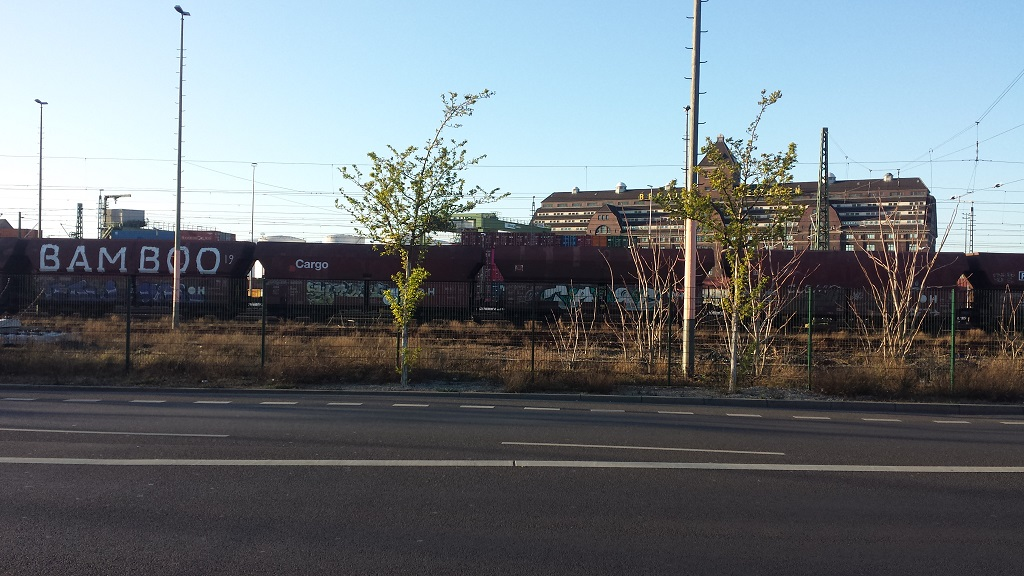
\includegraphics[width=1.0\textwidth]{img/inspiration/westhafen_view_postDurchgang.jpg}
   %\caption{Am Ende des Fu{\ss}g\"angerdurchgangs: typisch abgeranzte Hinterbahnhofshalde mit abgestelltem Lorenzug, irgendwer hat sich daran verewigt, aber niemanden interessiert es}
    %\label{img:inspiration_westhafen_view_postDurchgang}
    %\end{subfigure}
	%\caption{Fu{\ss}g\"angerdurchgang am Stadtgarten des ZK/U Gel\"andes, April 2020 zu einem CoVid-19 Ausgang im eigenen Revier}
	%\label{img:inspiration_westhafen_view_durchgang}
%\end{figure}


	
	\section{Szenische Ausgestaltung}
\label{sec:diorama}



\subsection{Geb\"aude}

Durch die Kindheit und Platten im famili\"aren Umfeld lag die Pr\"agung tendenziell auf romantischen Motiven in den Voralpen.
Herstellerseitig lag somit ein tiefer Bezug zu den Firmen
\textit{Faller}\footnote{Faller ist ein eingetragender Markenname der Faller GmbH. Alle Angaben zum Sortiment spiegeln die pers\"onlichen Ansichten des Autors wider und sind in keinster Weise despektierlicher Natur.} und
\textit{Vollmer}\footnote{Vollmer ist ein eingetragender Markenname der Vollmer GmbH \& Co. KG i.~L., inzwischen durch die Viessmann Modelltechnik GmbH vertrieben. Alle Angaben zum Sortiment spiegeln die pers\"onlichen Ansichten des Autors wider und sind in keinster Weise despektierlicher Natur.} vor.
Leider sind die neuen Bundesl\"ander, insbesondere abseits der Mittelgebirge, in den Sortimenten nicht so gut vertreten.
Die Idee war daher, auf Modellbahnb\"orsen sammeln zu gehen und ggf. sogar selbst zu basteln.
Ein erster Besuch auf einer Bahnb\"orse in Berlin war allerdings etwas ern\"uchternd und die F\"ahigkeit zu hochpr\"zisem Basteln ist eigentlich auch nicht vorhanden.

Ein gro{\ss}er Lichtblick war das Auffinden der Firma
\textit{Auhagen}\footnote{Auhagen ist ein eingetragender Markenname der Auhagen GmbH. Alle Angaben zum Sortiment spiegeln die pers\"onlichen Ansichten des Autors wider und sind in keinster Weise despektierlicher Natur.}.
In Sachsen beiheimatet, liegt hier ein ganz deutlicher Bezug zu den neuen Bundesl\"andern vor.
Das H0-Sortiment weist eine hervorragende F\"ulle auf.
In Spur N ist es schon ein bisschen \"ubersichtlicher, aber das wichtigste ist vorhanden.



\subsubsection{Bahnhofsgeb\"aude Granitz}

Das Hauptgeb\"aude des Bahnhofs ist ein f\"ur die Region typischer, repr\"asentativer Backsteinbau.
\begin{itemize}
	\item[] Hersteller:~Auhagen
	\item[] Bezeichnung:~Bahnhof Neupreu{\ss}en
	\item[] Artikel-Nr.:~14485
\end{itemize}

\subsubsection{Bahnsteige in Granitz}

Prim\"are, \"uberdachte Bahnsteige:
\begin{itemize}
	\item[] Hersteller:~Auhagen
	\item[] Bezeichnung:~Bahnsteig
	\item[] Artikel-Nr.:~14481
\end{itemize}
Ggf. auf Bahnsteig Gleis IV/V verl\"angert um moderenen, nachger\"usteten, sekund\"aren Bahnsteig:
\begin{itemize}
	\item[] Hersteller:~Auhagen
	\item[] Bezeichnung:~Bahnsteig
	\item[] Artikel-Nr.:~14459
\end{itemize}

Nicht \"uberdachte Verl\"angerungungen durch gefertigte Bahnsteigkanten und selbstgemachter Verf\"ullung der Bahnsteigfl\"achen \hl{Holz/Pappe, Gips?}.
\begin{itemize}
	\item[] Hersteller:~Auhagen
	\item[] Bezeichnung:~Bahnsteigkanten
	\item[] Artikel-Nr.:~44631
\end{itemize}

\subsubsection{Bahnsteige in Granitz-Walddorf}

\"Uberdachte Bahnsteige:
\begin{itemize}
	\item[] Hersteller:~Auhagen
	\item[] Bezeichnung:~Bahnsteig
	\item[] Artikel-Nr.:~14459
\end{itemize}

Nicht \"uberdachte Verl\"angerungungen durch gefertigte Bahnsteigkanten und selbstgemachter Verf\"ullung der Bahnsteigfl\"achen \hl{Holz/Pappe, Gips?}.
\begin{itemize}
	\item[] Hersteller:~Auhagen
	\item[] Bezeichnung:~Bahnsteigkanten
	\item[] Artikel-Nr.:~44631
\end{itemize}



\subsubsection{Wohngeb\"aude in Granitz}

Viele B\"urger sind in Wohnplatten untegebracht:
\begin{itemize}
	\item[] Hersteller:~Auhagen
	\item[] Bezeichnung:~Mehrfamilienhaus
	\item[] Artikel-Nr.:~14472
\end{itemize}
Diese Wohnplatte eignet sich auch f\"ur die Darstellung verlassener, im Verfall befindlicher Wohn- oder Kasernenanlagen.
Aus zwei erworbenen Artikeln sind die Fassaden f\"ur zwei gesunde und ein alternatives, verlassenes Wohnobjekt verf\"ugbar.
Die Seitenwand und ein Flachdach des verlassenen Hauses kann mit \hl{Holz/lackierter Pappe} nachgebaut werden.

\begin{itemize}
	\item[] Hersteller:~
	\item[] Bezeichnung:~
	\item[] Artikel-Nr.:~
\end{itemize}

\begin{itemize}
	\item[] Hersteller:~
	\item[] Bezeichnung:~
	\item[] Artikel-Nr.:~
\end{itemize}

\begin{itemize}
	\item[] Hersteller:~
	\item[] Bezeichnung:~
	\item[] Artikel-Nr.:~
\end{itemize}
	
	\section{Hardware}
\label{sec:hardware}

ToDo

\subsection{Handbetrieb}
\label{sec:manual_operation}



\subsection{Computergest\"utzter Betrieb}
\label{sec:pc_operation}



\subsection{Ferngesteuerter Betrieb}
\label{sec:remote_operation}

Der ferngesteuerte Betrieb (Remotesteuerung) meint hier eine Steuerung im Sinne von Kap.~\ref{sec:pc_operation} von einem beliebigen, geeigneten Ger\"at aus.
Hier steht das Smartphone als intuitivste und wahrscheinlich sinnvollste Anwendungsm\"oglichkeit f\"ur das Beispiel Pate.

Die Hardware an der Anlage bleibt in diesem Zuge unver\"andert, entspricht also der in Kap.~\ref{sec:pc_operation} beschriebenen.
Die Software entspricht ebenfalls der eigentlich verwendeten, die nachfolgend in Kap.~\ref{sec:software} vorgestellt wird.
F\"ur die Remotesteuerung ist dann insbesondere Kap.~\ref{sec:remote_irc} relevant.

Eigene, angepasste Hardware ist demzufolge nicht notwendig - allenfalls die hauseigene LAN oder WLAN Infratruktur.
	
	\section{Software}
\label{sec:software}

Softwareseitig handelt es sich um eine Eigenentwicklung, den DWRasp-Rail-Controller (DWRRC).
Dieser setzt auf einer weiteren Eigenentwicklung auf, n\"amlich dem Projekt DWRasp-on-PsiCore.
Die Git-Projekte zu beiden Projekten sind unter folgenden Links verf\"ugbar:
\begin{itemize}
	\item \textit{https://github.com/dwoelki/DWRasp-on-PsiCore}
	\item \textit{https://github.com/dwoelki/DWRasp-Rail-Controller}
\end{itemize}
Zu beachten ist, dass das DWRasp-on-PsiCore Projekt selbst Drittsoftware einbindet.
Dabei handelt es sich um das $\Psi$-Core, das am Institut f\"ur Luft- und Raumfahrt der Technischen Universit\"at Berlin (ILR) entwickelt wurde.
Das $\Psi$-Core ist die Engine der ILR-hauseigenen Simulationsumgebung IPSM (Interface for Performance and Secondary Air System Modeling) \cite{Woe14}, \cite{Woe19c}.
Zuf\"alligerweise sind der Sch\"opfer bzw. Hauptentwickler von IPSM sowie der Sch\"opfer von Granitz ein und dieselbe Person.

Der Quellcode aller genannten Projekte ist fast vollst\"andig in der Programmiersprache Java geschrieben und objektorientiert.
Das $\Psi$-Core sowie alle darauf aufbauenden Anwendungen, die ich schreibe (also auch DWRRC) sind \"ublicherweise stark modularisiert.
Im vorliegenden Fall ist die Modularisierung aber linear und somit recht leicht nachvollziehbar.
Als bevorzugte IDE wurde Netbeans IDE (sowohl in vor- als auch zu-Apache Zeiten) genutzt.
Die aus den Projekten erzeugten Bibliotheken entsprechen somit \"ublicherweise Modulen/Plugins mit entsprechenden Netbeans Spezifikationen.
Am einfachsten ist daher die Adaption der Projekte direkt mit Netbeans als frei verf\"ugbare IDE.
Eine Konvertierung auf andere IDEs bzw. Extrahierung des ben\"otigten Quellcodes bedeutet f\"ur den ge\"ubten Programmierer aber nat\"urlich kein gro\"ser Aufwand.





\subsection{Hardwareansteuerung \"uber GPIO}
\label{sec:gpio}



\subsection{Remotesteuerung \"uber IRC}
\label{sec:remote_irc}

	\begin{thebibliography}{laengste Breite}

\bibitem[Gee17]{Gee17} Geering, F. (2017). Vom Kreisverkehr zum Betriebserlebnis. URL: \textit{http://k.f.geering.info}, Abruf vom 21. Mai 2020.

\bibitem[W\"ac07]{W\"ac07} W\"achter, G. (2007). Railroad Construction Pack Trackplanner. URL: \textit{http://www.trackplanner.de}, Abruf vom 21. Mai 2020.

\bibitem[Woe14]{Woe14} Woelki, D. and Peitsch, D. (2014). Modellierung variabler Sekund\"arluftsysteme zur Bewertung ihrer Auswirkungen auf das Gesamtsystem Gasturbine. In: \textit{Deutscher Luft- und Raumfahrtkongress 2014}. Augsburg. \textit{https://nbn-resolving.org/urn:nbn:de:101:1-2015012312500}

\bibitem[Woe19c]{Woe19c} Woelki, D. and Peitsch, D. (2019). A Framework for Applied Component Zooming in Gas Turbines. In: \textit{Deutscher Luft- und Raumfahrtkongress 2019}. Darmstadt. \textit{https://doi.org/10.25967/490174}

	
\end{thebibliography}


\setcounter{section}{0}
\renewcommand*\theHsection{\Alph{section}}
\renewcommand*\thesection{\Alph{section}}

  \setcounter{section}{0}
\renewcommand*\theHsection{\Alph{section}}
\renewcommand*\thesection{\Alph{section}}


\section{Appendix}
\label{sec:appendix}

ToDo
	
	\section{Digital Appendix}
\label{sec:digitalAppendix}

\subsection{Gleispl\"ane f\"ur Trackplanner}

Die angeh\"angten \textit{.glp} Dateien enthalten Gleispl\"ane zur Bearbeitung mit der Software Trackplanner \cite{W\"ac07}.
Die Dateibenennung enth\"alt jeweils ein Datum im Format \textit{YYYY-MM-DD} ($Y$~=~Jahr, $M$~=~Monat, $D$~=~Tag).

\end{document}
